%% =====================================================================
%% Bell-Decomposition Quantum Kernels for Land Cover Classification
%%
%% Original manuscript submitted to Quantum Machine Intelligence (Springer).
%% Content transcribed verbatim from paper_revised_Orig.pdf.
%% =====================================================================
\documentclass[pdflatex,sn-mathphys]{sn-jnl}

\usepackage{graphicx}
\usepackage{multirow}
\usepackage{amsmath,amssymb,amsfonts,amsthm}
\usepackage{mathrsfs}
\usepackage{booktabs}
\usepackage{hyperref}
\usepackage{url}
\usepackage{xcolor}
\usepackage[para]{manyfoot}
%% orcidlink draws the canonical green ORCID iD symbol via TikZ and links to
%% the ORCID record; no external Orcidlogo.eps required.  Auto-installed by
%% MiKTeX; shipped with TeX Live since 2021.
%%
%% Note: the Springer sn-jnl class pre-defines \orcidlogo (expecting an
%% external Orcidlogo.eps file).  We release that name so orcidlink can
%% redefine it with its TikZ implementation; orcidlink supplies the
%% user-level macro \orcidlink{<bare-id>} we use below.
\let\orcidlogo\relax
\usepackage{orcidlink}

%% This version of the Springer Nature sn-jnl class (2024+) sets the
%% publication year via the journal production system, so \jyear is no
%% longer a user-level command.  Older docs use \jyear{<year>}.

%% Springer sn-jnl defines its own theorem styles (thmstyleone, etc.) only
%% if amsthm is already loaded at class-load time.  Because the user
%% preamble loads amsthm AFTER \documentclass, those styles never fire,
%% so we use amsthm's standard styles, which match Springer's general
%% appearance for theorem-like environments.
\theoremstyle{plain}
\newtheorem{theorem}{Theorem}
\newtheorem{proposition}{Proposition}
\newtheorem{lemma}{Lemma}

\theoremstyle{remark}
\newtheorem{remark}{Remark}

\theoremstyle{definition}
\newtheorem{definition}{Definition}

\raggedbottom

\begin{document}

\title[Bell-Decomposition Quantum Kernels]{Bell-Decomposition Quantum Kernels: A Multi-Scale Benchmark on Earth Observation and Beyond}

\author[1]{\fnm{Prajwal S.} \sur{Gaikwad}\,\orcidlink{0000-0003-0805-9130}}
\author*[1]{\fnm{Prathamesh Balasaheb} \sur{Kadam}\,\orcidlink{0009-0006-9211-4647}}\email{prathameshkadam130404@gmail.com}
\author[1]{\fnm{Shreyas Subhash} \sur{Raut}\,\orcidlink{0009-0007-8900-9560}}
\author[1]{\fnm{Tejas Uttam} \sur{Shitole}\,\orcidlink{0009-0004-2175-8723}}

\affil*[1]{\orgdiv{Department of Artificial Intelligence and Data Science},
\orgname{AISSMS Institute of Information Technology, Pune},
\country{India}}

\abstract{
We introduce the Bell-decomposition family of two-qubit feature maps, unifying the singlet-only Self-Regulating Quantum Feature Map (SRQFM) and the four-Bell-sector Bell-Spectrum Coupling Map (BSCM) under an adjustable prior. The family sits inside the canonical two-body Pauli-rotation feature-map framework of Suzuki et al.\ (QMI 2020); within that framework we prove two closed-form structural identities specific to the Bell-projector construction: a tight prior-independent bound $|\alpha|\le 1/2$ on every per-pair Pauli coefficient, and $\alpha_{ZZ}\equiv 0$ for the uniform prior, making BSCM-uniform strictly Pauli-orthogonal to any SRQFM-style $ZZ$ generator. A single hyperparameter $\tau$, locked once at $n=8$, transfers operationally to $n=14$ and $n=16$. We report four findings. \textbf{(i) Architectural advantage}: at 16 qubits and $N=10{,}000$ the Bell-decomposition projected kernels add $+0.167$--$+0.170$ macro-F1 over commuting $ZZ$-PQK on So2Sat LCZ42 (17 classes) and $+0.097$--$+0.108$ on EuroSAT (10 classes); Holm-corrected Wilcoxon $p=0.0078$ on both. \textbf{(ii) Domain-agnostic}: the gap is positive on every split across four UCI datasets (largest $+0.646$ accuracy on the 26-class Letter task, whose 16 features match $n=16$) and on a transverse-field Ising-model phase-classification benchmark. \textbf{(iii) Noise-robust}: under density-matrix simulation at $n=8$ the gap remains $+0.133$--$+0.136$ across $p\in\{0,0.001,0.005,0.01\}$. \textbf{(iv) Concentration on real data}: a 14-qubit BSCM build at $N=800$ and a 16-qubit depth scan at $N=2{,}000$ reproduce the Thanasilp et al.\ concentration signature on real multi-class remote-sensing data. The Bell-decomposition kernels match but do not exceed tuned classical RBF-SVM at any scale tested, consistent with recent theory (Canatar et al.; Fl{\'o}rez-Ablan, Roth and Schnabel) and prior empirical work (Bowles et al.; Schnabel and Roth).}

\keywords{Quantum kernel methods, Pauli decomposition, Bell-state feature maps, Projected quantum kernels, Exponential concentration, Land cover classification}

\maketitle

%% =====================================================================
\section{Introduction}\label{sec:intro}
%% =====================================================================

Quantum machine learning (QML) has been studied as a possible route to computational advantage in pattern recognition. Among the proposed approaches, kernel methods are particularly clean: a parameterised unitary $U(x)$ embeds a classical input into a quantum feature space, the fidelity kernel $K(x,x')=|\langle 0|U^\dagger(x')U(x)|0\rangle|^2$ defines a similarity function, and a downstream classical Support Vector Machine (SVM) does the learning \cite{havlicek2019,schuld2019}. Theoretical analysis has shown that for problems whose hardness matches the circuit's inductive bias, quantum kernels can in principle outperform any efficient classical kernel \cite{liu2021}. However, for typical applied datasets this match is rare, and recent benchmarks --- Bowles \emph{et al.}\ \cite{bowles2024} on 160 datasets generated from six binary-task families, Schnabel \& Roth \cite{schnabel2025} on 64 datasets in QMI 2025 --- consistently fail to find a robust advantage over tuned classical baselines such as the radial-basis-function (RBF) kernel SVM.

Land cover classification from satellite imagery is a stringent applied benchmark: So2Sat LCZ42 \cite{zhu2020} contains $400{,}673$ multimodal Sentinel-1 (synthetic-aperture-radar, SAR) and Sentinel-2 (multispectral optical) patches across 42 cities and 17 Local Climate Zone (LCZ) classes, with class fractions ranging from $0.7\%$ to $13.6\%$ in our subsample; EuroSAT \cite{helber2019} contains $\sim\!27{,}000$ Sentinel-2 patches in 10 classes. Despite growing QML interest in Earth observation \cite{rodriguez2025}, no published kernel-method study we are aware of has evaluated multiple quantum kernel architectures on these benchmarks at 16 qubits with $N=10{,}000$ under a fixed-pool, multi-seed, $C$-tuned protocol --- existing QK benchmarks (Schnabel \& Roth \cite{schnabel2025}, $M\!=\!240$ training / $M'\!=\!60$ test points on each of 64 mostly-synthetic datasets, $n\!\le\!15$; Bowles \emph{et al.}\ \cite{bowles2024}, 160 datasets generated from six binary-task families, $n\!\le\!18$; Rodriguez-Grasa \emph{et al.}\ \cite{rodriguez2025}, $N\!=\!1{,}800$ binary solar-panel detection at $n\!\le\!8$) operate at smaller scale or different class structure. This paper supplies the evaluation at the scale our contribution requires.

The technical content is organised around a single design principle. The two-qubit encoded state $|\psi(x_i)\rangle|\psi(x_j)\rangle$ can be written in the Bell basis as a weighted sum of four projectors, $|\Phi^\pm\rangle\!\langle\Phi^\pm|$ and $|\Psi^\pm\rangle\!\langle\Psi^\pm|$, with weights determined by the inputs. Choosing which weights are activated as data-dependent gate angles maps out a structured design space. Two natural choices populate this space: SRQFM (singlet-only, equivalent to a particular $ZZ$-fidelity construction) and BSCM (all four sectors with an adjustable prior). The two constructions are theoretically distinct --- the \emph{uniform} BSCM preset is provably Pauli-orthogonal to SRQFM in the per-pair generator (\S\ref{sec:bscm}) --- but turn out to be empirically indistinguishable in macro-F1 at $N\le 2000$. The interesting behaviour appears at the boundaries: at 14 qubits both members regress toward concentrated kernels with weakened class structure; at 16 qubits and $N=10{,}000$ the Bell-decomposition \emph{projected} quantum kernels (BSCM-PQK family) add $+0.167$ to $+0.170$ macro-F1 over the canonical Standard $ZZ$-PQK on So2Sat and $+0.097$ to $+0.108$ on EuroSAT, demonstrating that non-commuting gate geometries substantially outperform the canonical commuting $ZZ$ architecture within the projected quantum kernel framework. On four standard UCI datasets (Digits, Breast Cancer, Letter Recognition with 16 features exactly matching $n=16$, and Wine as a 13-feature padding boundary case) BSCM-uniform-PQK exceeds Standard-$ZZ$-PQK on every dataset (gap $+0.546$ on Digits, $+0.289$ on Breast Cancer, $+0.646$ on Letter, $+0.348$ on Wine), confirming that the architectural advantage is domain-agnostic; BSCM-PQK additionally \emph{matches} classical baselines within $\sim$2 percentage points on Digits and Breast Cancer.  All headline architectural-advantage numbers in this paper refer to the projected-kernel readout (Bloch-vector RBF) unless explicitly labelled \emph{fidelity} or \emph{FQK}; fidelity-kernel results for the same family appear in the smaller-scale $N\!\le\!2{,}000$ experiments E26/E32.

We make four claims:

\begin{enumerate}
  \item \textbf{Family.} The Bell-decomposition family unifies SRQFM and BSCM as Pauli-decomposition complements with a closed-form per-pair generator and provably bounded gate angles ($|\alpha|\le 1/2$ for the three priors evaluated in this paper, uniform / phi-only / psi-only; Theorem~\ref{thm:bscm-pauli}(a)).  A single hyperparameter $\tau$ controls the coefficient scale; the value $\tau=0.25$ locked from a 200-sample holdout at $n=8$ transfers operationally to $n=14$ and $n=16$ without re-tuning (\S\ref{sec:kernels}).
  \item \textbf{Architectural advantage.} At 16 qubits and $N=10{,}000$ on So2Sat LCZ42 and EuroSAT, the Bell-decomposition \emph{projected} kernels (BSCM-PQK family) add $+0.167$ to $+0.170$ macro-F1 over the canonical commuting Standard $ZZ$-PQK on So2Sat and $+0.097$ to $+0.108$ on EuroSAT, with Holm-corrected Wilcoxon $p = 0.0078$ on both datasets (the 10-split minimum achievable raw $p = 1/2^{9} \approx 0.002$).  Non-commuting $XX$, $YY$, $ZZ$ gate geometries materially outperform the single-axis $ZZ$ within the projected quantum kernel framework.
  \item \textbf{Domain-agnostic.} On four standard UCI tabular datasets --- Digits, Breast Cancer, Letter Recognition (16 features exactly matching $n=16$), and Wine (13 features, padded as a boundary case) --- and one intrinsically-quantum dataset (TFIM phase classification on 16-site ground states), BSCM-uniform-PQK exceeds Standard-$ZZ$-PQK by a positive margin on every dataset and every split.  Standard-$ZZ$-PQK collapses on every evaluated UCI dataset ($41.4\%$, $61.6\%$, $13.3\%$, $40.7\%$ accuracy on Digits, Breast Cancer, Letter, Wine, versus BSCM's $96.0\%$, $90.5\%$, $77.9\%$, $75.6\%$), with the largest architectural gap $+0.646$ accuracy on the 26-class Letter task.  BSCM-vs-classical: $\le$2 percentage points on Digits and Breast Cancer; $\sim$8 pts behind RBF on the 26-class Letter task; $\sim$21 pts on Wine, attributable to the $n=16$-vs-13-feature circuit-width artefact analysed in \S\ref{sec:domain-gen}.  The Earth-observation-specific-artefact reading is therefore ruled out.
  \item \textbf{Concentration on real data.} Two complementary measurements (real-data 14-qubit BSCM at $N=800$ on physics-Fisher-14; 16-qubit depth scan over $L\in\{2,\dots,10\}$ at $N=2{,}000$) exhibit the canonical Thanasilp concentration signature \cite{thanasilp2024} on real multi-class remote-sensing data, with all four kernel-health diagnostics moving in the predicted directions and a corresponding regression of macro-F1 toward tuned classical baselines.
\end{enumerate}

\noindent We make no claim of quantum advantage: at every scale tested, no Bell-decomposition kernel beats both tuned RBF-SVM and Random Forest; tuned Random-Fourier-Feature dequantisation \cite{rahimi2007} of the standard $ZZ$-FQK in fact \emph{exceeds} it by $+0.010$ macro-F1 on So2Sat PCA-8 at $D=512$ features (\S\ref{sec:rff}). This match-not-beat outcome is the expected regime under \cite{canatar2022,florezablan2025} and consistent with \cite{bowles2024,schnabel2025,rodriguez2025} at smaller scale.

\medskip
\noindent\textbf{What is new.}
Within the canonical two-body Pauli-rotation feature-map framework introduced by Suzuki \emph{et al.}\ \cite{suzuki2020}, we identify a specific Bell-projector construction --- a prior-weighted sum $H_{ij}=\sum_k p_k\,w_k\,2\,|B_k\rangle\!\langle B_k|$ over the four Bell-state projectors --- and prove two closed-form structural identities for it: \textbf{(a)} an explicit, tight bound $|\alpha_{XX}|, |\alpha_{YY}|, |\alpha_{ZZ}| \le 1/2$ on the per-pair Pauli coefficients, valid for all three priors evaluated in this paper and saturated on the input cube boundary; \textbf{(b)} the closed-form identity $\alpha_{ZZ}\equiv 0$ for the uniform prior, establishing strict Pauli-orthogonality between BSCM-uniform and any SRQFM-style $ZZ$-generator (Theorem~\ref{thm:bscm-pauli}).  In addition we report \textbf{(c)} an \emph{empirical regularity} that is not part of the theorem: a single scalar hyperparameter $\tau$, locked once from a 200-sample holdout at $n=8$, transfers operationally to $n=14$ and $n=16$ without re-tuning and produces both the predicted concentration regression (B2 / E37) and the headline architectural-gap result (E38) at the larger qubit counts (\S\ref{sec:kernels}; we do not claim $\tau=0.25$ is the argmax of KTA at $n=14$ or $n=16$, only that it remains operationally well-conditioned).  Property (c) is presented as an empirical observation throughout; it is consistent with --- and partially motivated by --- the bound in (a), but the scale transferability across qubit counts is verified experimentally, not proven.  Beyond the analysis, no prior study we are aware of has (d) measured the Thanasilp \cite{thanasilp2024} concentration regression on real multi-class remote-sensing data at 14 qubits with four simultaneously monitored kernel-health diagnostics, or (e) benchmarked multiple quantum kernel architectures at 16 qubits and $N=10{,}000$ on Earth-observation data under a fixed-pool, multi-seed, $C$-tuned protocol with $\tau$-locked hyperparameters and Holm-corrected significance tests.

\medskip
\noindent\textbf{Relation to recent benchmarks.}
Our finding that bandwidth-tuned PQKs match (but do not exceed) tuned classical RBF-SVM is the expected outcome of recent theory: Canatar \emph{et al.}\ \cite{canatar2022} proved that bandwidth selection is the dominant factor controlling generalisation in quantum kernel models and exhibited the bandwidth-tuned PQK $\to$ RBF correspondence on synthetic targets, and Fl{\'o}rez-Ablan, Roth and Schnabel \cite{florezablan2025} extended this picture to multiple data-encoding circuits, numerically demonstrating that optimal bandwidth tuning makes fidelity and projected quantum kernels statistically resemble RBF kernels across classification tasks. Empirical benchmarks have reached the same conclusion at smaller scale (\cite{schnabel2025}, 64 datasets, $M\!+\!M'\!=\!300$ points per dataset, $n\!\le\!15$; Bowles \emph{et al.}\ \cite{bowles2024}, 160 datasets from six binary-task families, $n\!\le\!18$; Rodriguez-Grasa \emph{et al.}\ \cite{rodriguez2025}, neural quantum kernels $\approx$ Random Forest on a binary EO task at $n\!\le\!8$, $N\!=\!1{,}800$). Our contribution is therefore not a new finding of \emph{whether} quantum kernels match classical, but: (i) the Bell-decomposition family of fidelity feature maps and the quantum-vs-quantum advantage of non-commuting gate geometries over the canonical $ZZ$ architecture, (ii) directly measured concentration regression on real multi-class data at 14 qubits, and (iii) domain-generalisation evidence showing that the architectural advantage is not specific to Earth observation, and (iv) a fixed-protocol multi-class Earth-observation benchmark at 16 qubits and $N=10{,}000$ that, to our knowledge, is the largest of its kind.

%% =====================================================================
\section{Related Work}\label{sec:related}
%% =====================================================================

\paragraph{Quantum kernel theory.}
Havl{\'\i}{\v{c}}ek \emph{et al.}\ \cite{havlicek2019} introduced the $ZZ$ Feature Map. Liu \emph{et al.}\ \cite{liu2021} proved an exponential advantage for a discrete-log task under specific hardness assumptions. Huang \emph{et al.}\ \cite{huang2021} proposed the geometric difference $g(K_q,K_c)$ as a separation diagnostic and showed advantage requires both $g\!\gg\!1$ and positive $\Delta$KTA. Schuld \cite{schuld2021} showed angle-encoded kernels are Fourier-series approximations whose expressibility beyond classical kernels requires entanglement.

\paragraph{Concentration and projected kernels.}
Thanasilp \emph{et al.}\ \cite{thanasilp2024} proved that fidelity kernels with global observables undergo \emph{exponential concentration}: off-diagonal entries converge exponentially in qubit count to a constant, eliminating discriminative structure. The Projected Quantum Kernel (PQK) \cite{huang2021} extracts single-qubit Bloch expectations and applies an RBF on the resulting low-dimensional embedding; Shaydulin \& Wild \cite{shaydulin2022} suggested CV-KTA bandwidth selection, which we adopt. Heyraud \emph{et al.}\ \cite{heyraud2022} analysed noisy quantum kernel machines and showed that decoherence and dissipation act as an \emph{implicit regularisation}, controlling the effective kernel rank and bounding the generalisation error via the average purity of the encoded states --- a result we use in our noise-robustness analysis (\S\ref{sec:aux-results}). Fl{\'o}rez-Ablan, Roth and Schnabel \cite{florezablan2025} formalised the conditions under which bandwidth-tuned quantum kernels become statistically indistinguishable from classical kernels.

\paragraph{Benchmarking.}
Bowles \emph{et al.}\ \cite{bowles2024} found classical models match or exceed twelve QML models on 160 datasets generated from six binary-classification task families, with circuits up to $n\!=\!18$ qubits. Schnabel \& Roth \cite{schnabel2025} reached the same conclusion across 64 datasets in five families ($M\!=\!240$ training / $M'\!=\!60$ test points each, $n\!\le\!15$ qubits) and $\sim\!20{,}000$ trained models covering both classification and regression in QMI 2025. Rodriguez-Grasa \emph{et al.}\ \cite{rodriguez2025} reported \emph{competitive but not superior} neural quantum kernel performance on binary solar-panel detection (Bradbury \emph{et al.}\ dataset) at up to $n\!=\!8$ qubits and $N\!=\!1{,}800$ training points in MLST 2025.
Table~\ref{tab:scale-compare} places the present study in context. None of the cited benchmarks combines multi-class classification ($K\ge 10$), $n=16$ qubits, and $N=10{,}000$ samples in a fixed-protocol study on Earth-observation data; our work fills that gap.

\begin{table}[htbp]
\caption{Scale comparison of recent fixed-protocol quantum-kernel benchmarks. $n$=qubits (maximum reported), $N$=pool size, $K$=number of classes, EO=Earth observation. Our study (bottom row, separated by a double-rule) is the only one combining $n\ge 16$, $N\ge 10{,}000$, and $K\ge 10$ on EO.}
\label{tab:scale-compare}
\footnotesize
\setlength{\tabcolsep}{3pt}
\begin{tabular}{@{}lcccl@{}}
\toprule
Study & $n$ & $N$ & $K$ & Domain \\
\midrule
Schnabel \& Roth \cite{schnabel2025}           & $\le 15$ & $300$        & 2     & Mixed tabular \\
Bowles et al.\ \cite{bowles2024}               & $\le 18$ & $\le 250$    & 2     & Mixed \\
Rodriguez-Grasa et al.\ \cite{rodriguez2025}   & $\le 8$  & $1{,}800$    & 2     & EO (solar) \\
\midrule
This work                                       & $16$     & $10{,}000$   & 10--17 & EO (So2Sat / EuroSAT) \\
\bottomrule
\end{tabular}
\end{table}

\paragraph{Bell- and Pauli-decomposition feature maps.}
Suzuki \emph{et al.}\ \cite{suzuki2020} introduced Pauli-rotation feature maps with arbitrary two-body generators of the form $H_{ij}=\sum_{P\in\{X,Y,Z\}^{\otimes 2}}\alpha_P\,P_iP_j$ and analysed their expressive power; that work is generator-agnostic by design and treats the Pauli coefficients $\alpha_P$ as an input choice.  What it does not provide are tight bounds on the achievable $\alpha_P$, identities that pin specific coefficients to zero, or a route to scale-stable hyperparameter discipline across qubit counts; those are subspace-specific questions.

\paragraph{Bell-projector construction.}
The contribution of this paper, within Suzuki's framework, is a specific construction of $H_{ij}$ as a non-negative-prior weighted sum of the four Bell-state projectors, $H_{ij}=\sum_k p_k\,w_k\,2\,|B_k\rangle\!\langle B_k|$, and a closed-form analysis of its resulting Pauli coefficients (Theorem~\ref{thm:bscm-pauli}, Appendix~\ref{appx:bscm}).  We emphasise that the theorem's proof technique is elementary --- substitution of the standard two-qubit Bell-Pauli identities (Lemma~\ref{lem:bell-pauli}) into the construction and collection of like terms; the contribution is the construction itself and the design-relevant identities it admits, not the proof technique.  This construction admits three properties not visible from the generic Pauli-rotation framework: (a) an explicit prior-independent tight bound $|\alpha_P|\le 1/2$, saturated on the boundary of $[0,\pi]^2$ (Theorem~\ref{thm:bscm-pauli}(a)), following from $w_k\in[0,1/2]$ and the $\{\pm 1/4\}$ projector coefficients of Lemma~\ref{lem:bell-pauli}; (b) the closed-form identity $\alpha_{ZZ}\equiv 0$ for the uniform prior $\boldsymbol{p}=(1,1,1,1)$ (Theorem~\ref{thm:bscm-pauli}(b)), from the sector-sum identities $w_{\Phi^+}+w_{\Phi^-}=w_{\Psi^+}+w_{\Psi^-}=1/2$; and (c) an empirically scale-stable single hyperparameter $\tau$, locked at $n=8$ and operational at $n=14$ and $n=16$ without re-tuning (Tabs.~\ref{tab:b2}, \ref{tab:e37}, \ref{tab:e38}).  Properties (a) and (b) are proven; (c) is an empirical regularity consistent with (a), not a theorem.  The contribution is therefore a canonical four-point design space within Suzuki's framework --- with closed-form bounds, an orthogonality identity, and a scale-stable hyperparameter --- numerically verified by the unit-test suite (\texttt{tests/test\_proofs.py}, $10^{-8}$ tolerance).  SRQFM (singlet-only) and BSCM (four-sector with adjustable prior) are two specific points in this design space.

\paragraph{Inductive bias and bandwidth.}
K\"ubler \emph{et al.}\ \cite{kubler2021} showed angle-encoded quantum kernels possess a high-frequency inductive bias detrimental on smooth targets --- precisely the regime occupied by spectral remote-sensing features. Canatar \emph{et al.}\ \cite{canatar2022} proved bandwidth selection is critical for generalisation.

\paragraph{Remote sensing benchmarks.}
On So2Sat LCZ42 \cite{zhu2020}, deep CNN baselines (Sen2LCZ-Net \cite{qiu2020}, ResNeXt) reach $\sim\!61$--$70\%$ overall accuracy on the held-out cultural-10 test split using the full $32\!\times\!32$ image cube. EuroSAT \cite{helber2019} is essentially saturated by deep models ($\ge 98\%$ with ResNet-50). Tabular handcrafted-feature pipelines score lower; their interest is methodological --- they provide a controlled, low-dimensional setting in which kernel-vs-kernel separation can be measured cleanly.

%% =====================================================================
\section{Methods}\label{sec:methods}
%% =====================================================================

\subsection{Data and feature engineering}\label{sec:features}
We use two datasets. \textbf{So2Sat LCZ42} \cite{zhu2020}: training patches from the 32 culture-1 cities, 17 LCZ classes, fused Sentinel-1 SAR (8 channels) and Sentinel-2 multispectral (10 channels) imagery at $32{\times}32$ resolution. \textbf{EuroSAT (all-bands)} \cite{helber2019}: 13-band Sentinel-2 patches at $64{\times}64$ resolution, 10 land-cover classes. Quantum kernels at $n=8,14,16$ qubits encode one feature per qubit, so the principal feature-engineering choice is which $n$ scalar features to extract per patch.

\paragraph{Physics-8 (interpretable spectral / radar indices).}
For both datasets we compute eight physically-motivated indices as the spatial mean over each patch.

\noindent \emph{EuroSAT physics-8}, computed from Sentinel-2 bands $B_2$~(blue), $B_3$~(green), $B_4$~(red), $B_5$~(red-edge 1), $B_8$~(NIR), $B_{11}$~(SWIR1):
\begin{align*}
\mathrm{NDVI}  &= \frac{B_8 - B_4}{B_8 + B_4}, &
\mathrm{NDBI}  &= \frac{B_{11} - B_8}{B_{11} + B_8}, \\
\mathrm{NDWI}  &= \frac{B_3 - B_8}{B_3 + B_8}, &
\mathrm{BSI}   &= \frac{(B_{11}+B_4) - (B_8+B_2)}{(B_{11}+B_4) + (B_8+B_2)}, \\
\mathrm{SAVI}  &= \frac{1.5\,(B_8 - B_4)}{B_8 + B_4 + 0.5}, &
\mathrm{NDRE}  &= \frac{B_8 - B_5}{B_8 + B_5}, \\
\mathrm{MNDWI} &= \frac{B_3 - B_{11}}{B_3 + B_{11}}, &
\mathrm{EVI}   &= \frac{2.5\,(B_8 - B_4)}{B_8 + 6 B_4 - 7.5 B_2 + 1}.
\end{align*}

\noindent \emph{So2Sat physics-8} mixes Sentinel-2 indices (NDVI, NDBI, NDWI, BSI, SAVI, NDRE, MNDWI, EVI computed from the same Sentinel-2 band formulae above) with four Sentinel-1 SAR features computed from Lee-filtered VV and VH backscatter:
$\text{VV/VH ratio}=\mathrm{VV}/(\mathrm{VH}+\varepsilon)$,
$\text{SAR-total}=\mathrm{VV}+\mathrm{VH}$,
$\text{CrossPol}=\mathrm{VH}/(\mathrm{VV}+\varepsilon)$, and
$\text{PolCoh} = \sqrt{c_r^2+c_i^2}/\sqrt{\mathrm{VV}\cdot\mathrm{VH}+\varepsilon}$
where $(c_r, c_i)$ is the polarimetric covariance.

\paragraph{PCA-8 (statistical dimensionality reduction).}
8 leading components of Principal Component Analysis (PCA) on the standardised per-patch mean values of all available bands ($13$ for EuroSAT; $18$ for So2Sat) plus second-order textures (variance, GLCM-contrast where applicable). The PCA is fit on a held-out background set (samples not in the evaluation pool) to avoid test-set leakage.

\paragraph{Fisher-14 and Fisher-16 (top-rank feature selection).}
For 14- and 16-qubit experiments we rank the full pool of available features by the Fisher-ratio criterion $F_k = \tfrac{\sigma^2_{\text{between-class},k}}{\sigma^2_{\text{within-class},k}}$ on the held-out background set, then keep the top-14 (B2, the 14-qubit concentration-regression diagnostic) or top-16 (E37 / E38). \textbf{So2Sat}: the candidate pool is the 16-element set defined by \texttt{scripts/test\_physics\_classical.py:extract\_16\_features}, namely the 8 Sentinel-2 indices (NDVI, NDBI, NDWI, BSI, SAVI, NDRE, MNDWI, EVI), 4 SAR ratios (VV/VH, total backscatter, cross-pol, PolSAR coherence), 2 SAR dB features ($10\log_{10}$ of Lee-filtered VH and VV intensity), and 2 spatial-variance ``texture'' features (VV-channel pixel-std and per-pixel NDVI std).  The \emph{Fisher-selected physics-8} of E26 / E28 / E32 selects 8 of these 16 with a modality-balance constraint ($\ge 2$ SAR, $\ge 2$ optical) implemented in \texttt{src/attention\_kernel.py:select\_features\_by\_fisher}.  \textbf{EuroSAT}: the candidate pool is the union of the 8 physics indices and the 13 raw Sentinel-2 band means (21 candidates); the Fisher-rank top-16 is selected without any modality constraint, so the chosen 16 are whatever happens to score in the top-16 by Fisher and may exclude some physics indices if their between-class variance ranks lower than a raw band's.

\noindent\emph{NDVI vs NDVI-texture}: NDVI (feature 1) is computed as $(B_8^\text{mean} - B_4^\text{mean})/(B_8^\text{mean} + B_4^\text{mean})$, the normalised difference of the patch-averaged NIR and Red bands.  NDVI-texture (feature 16) is the spatial standard deviation of the per-pixel NDVI computed pixel-by-pixel within the patch.  These are mathematically distinct objects (NDVI of the mean is not the mean of NDVI); we list both, with the convention that ``NDVI'' alone always refers to feature 1 unless explicitly qualified as ``texture''.

\paragraph{Encoding scaling.}
The pipelines use one of two normalisation schemes, both fit strictly on a held-out background (or training fold) and applied to the evaluation pool.  Quantum encoding always lands in $[0, \pi]$; classical baselines see the standardised features without the min-max step.

\begin{itemize}
\item[(P)] \emph{Percentile-clip $\to$ MinMax[0, $\pi$]}, used by the So2Sat physics pipelines (E26 / E28 / E32 / B2 / E37 / E38-So2Sat) and the raw-band auxiliary.  Per feature, the 1st and 99th percentiles of the background set define the clipping bounds; values outside are clipped to those bounds and then linearly scaled to $[0, \pi]$.  This is robust to PCA / Fisher outliers that would otherwise compress 99\% of the data into a tiny sub-range of $[0, \pi]$.
\item[(S)] \emph{StandardScaler $\to$ MinMax[0, $\pi$]}, used by the EuroSAT 10k pipeline (E38-EuroSAT) and by E43 / E49 inside the cross-validation loop.  Zero-mean / unit-variance fit on the train split, then min-max to $[0, \pi]$ on the same.  Outlier handling is left to the StandardScaler's variance normalisation.
\end{itemize}

The AE-16 pipeline (E42) combines both: a StandardScaler on the 16-dimensional AE bottleneck output, followed by a 1st/99th-percentile clip, followed by min-max to $[0, \pi]$ (\texttt{scripts/extract\_so2sat\_ae16.py}).  None of these conventions changes the architectural-advantage comparison \emph{within} a single experiment because both quantum kernels in any given experiment use the same scheme; the conventions only matter if absolute numbers are compared across experiments, in which case the within-pool / cross-pool distinction of the previous paragraph applies.

\paragraph{Pairwise correlation diagnostic.}
Figure~\ref{fig:feature-corr} displays the Pearson correlation matrix of the eight physics features on each dataset. So2Sat physics-8 has $12$ of $28$ pairs with $|\rho|>0.85$; EuroSAT physics-8 has $11$. The strongest EuroSAT pairs are NDVI--NDRE ($+0.989$), SAVI--EVI ($+0.989$), and NDVI--SAVI ($+0.963$) --- four near-duplicate vegetation indices. These high correlations interact with the per-pair Pauli generator in a kernel-architecture-dependent way (\S\ref{sec:feature-effect}).

\begin{figure}[htbp]
\centering
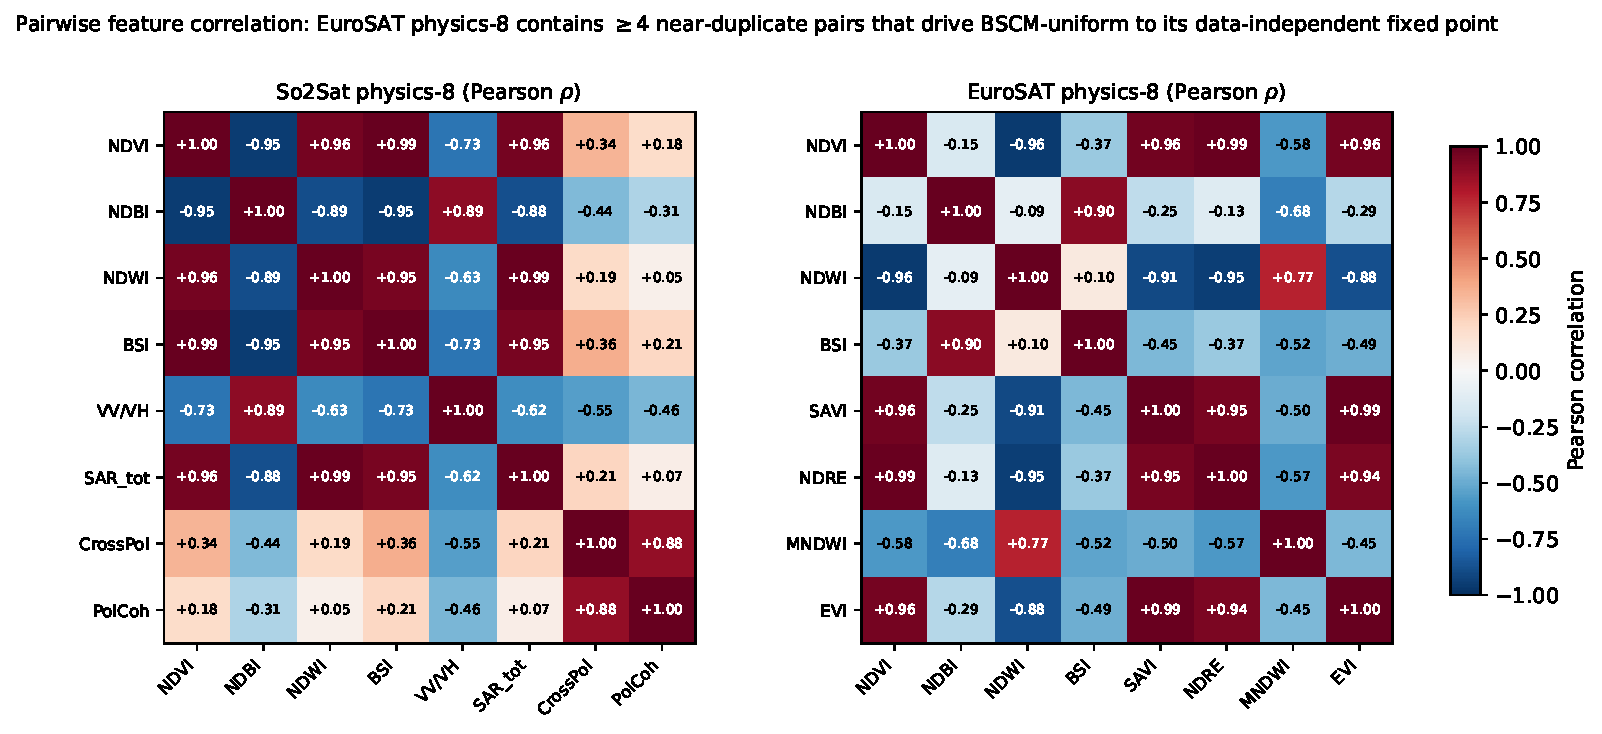
\includegraphics[width=0.95\linewidth]{figures/fig_feature_correlation.pdf}
\caption{Pairwise Pearson correlation of physics-8 features on So2Sat (left) and EuroSAT (right). Cell colour encodes $\rho\in[-1,+1]$. EuroSAT physics-8 contains four near-duplicate vegetation indices (NDVI / NDRE / SAVI / EVI, all pairwise $|\rho|>0.96$), so the BSCM-uniform per-pair generator on those four features produces a kernel sub-structure with reduced discriminative content. So2Sat physics-8 contains a similar density of high-$|\rho|$ pairs but does not exhibit the same effect, indicating that correlation density is necessary but not sufficient.}
\label{fig:feature-corr}
\end{figure}

\paragraph{Fixed-pool protocol.}
Following the recommendations of \cite{schnabel2025} we use a fixed evaluation pool of size $N_{\text{pool}}$ (e.g.\ $1{,}800$ for E32; $10{,}000$ for E38) sampled once with a master seed, then drawn into \textbf{train/test splits} by \texttt{StratifiedShuffleSplit(random\_state=42, test\_size=0.30)} with \texttt{n\_splits=5} for E26/E32 and \texttt{n\_splits=10} for E38, so that all methods on a given experiment see the identical sequence of splits. Feature scaling and PCA are fit on the training split only. Quantum kernels are precomputed on the full pool and submatrix-indexed per fold to amortise the $O(N^2)$ cost; this makes the move from 5 to 10 splits in E38 cost only the SVM evaluation step ($\sim$minutes), not a re-extraction of Bloch vectors.

\paragraph{Within-pool versus cross-pool comparisons.}
A single fixed pool defines a within-pool experiment: all kernels and baselines on that pool see identical sample identities and identical train/test split sequences, so pairwise comparisons within the pool are unaffected by sampling variance.  Cross-pool comparisons are different: tuned RBF-SVM macro-F1 on independent $N\!\approx\!1{,}800$ stratified draws from the same dataset distribution can differ by $\sim$0.05 F1 (E26 reports $0.518\pm 0.020$; E32, on a different fixed pool, reports $0.465\pm 0.028$ for the same RBF estimator on the same dataset).  We substantiate this claim with a direct measurement: 50 stratified resamples of size $N=1{,}800$ drawn (without replacement) from the same physics-16 superset that E26 / E32 use, each followed by the identical E26 RBF-tuning protocol (single 70/30 stratified split at seed = 42, grid-CV over $C$ and $\gamma$).  The empirical distribution of tuned-RBF macro-F1 across the 50 resamples has mean $0.5229$, std $0.0214$, range $[0.480, 0.575]$ (max $-$ min $= 0.095$), and percentile $95\%$ band $[0.484, 0.567]$ (script: \texttt{experiments/audit\_pool\_variance\_rbf.py}; result: \texttt{results/pool\_variance\_rbf/rbf\_pool\_variance.json}).  The E26 Pool A value ($0.518$) lies near the centre of this distribution; the E32 Pool B value ($0.465$) lies below the empirical $95\%$ lower bound but within the observed max $-$ min range --- the two pools are at the more dispersed end of the resampling distribution but neither is an outlier in absolute terms.  This is benchmark-stability variance at small $N$, independent of any kernel-specific effect.  Throughout the paper, comparisons within a single experiment (within-pool) are reported as primary statistical evidence, and comparisons across experiments with disjoint pools (cross-pool) are reported as indicative only.  The $N=10{,}000$ pool used by the headline E38 experiment damps this variance to the $\sim$0.005 F1 level (10 splits, fixed pool).

\subsection{Quantum hardware and simulation}
All quantum kernels are evaluated on noiseless statevector simulators in PennyLane (\texttt{lightning.qubit} for the production 16-qubit runs E37/E38; \texttt{default.qubit} for the smaller E42 / E43 / E44 / E46 protocols) using gate sets compatible with IBM Quantum hardware (controlled-NOT (CNOT), Pauli single-qubit rotations $R_X, R_Y, R_Z$). Noise robustness (Exp.\ E3) is studied by post-hoc depolarising noise injection at $p\in [0,0.05]$ on the FQK gram. We do not perform native-hardware execution; the implications are discussed in Sec.~\ref{sec:limits}.

\paragraph{Use of generative-AI tools.}
In line with the Springer Nature generative-AI authorship policy, we disclose that a large language model assistant (Anthropic Claude) was used as a supervised productivity aid during this work.  Its role was limited to two well-bounded tasks: (i) scaffolding boilerplate code (data-loading, JSON serialisation, figure-generation utilities, and command-line plumbing for the per-experiment scripts), which the authors then audited line-by-line, modified, and re-ran end-to-end on their own hardware; and (ii) copy-editing and formatting assistance for the LaTeX manuscript --- consistency checks across the per-experiment JSON result files and the in-text numerical citations, table layout, and prose tightening.
%
All conceptual and scientific decisions --- the research question, the choice of feature-map family, the experimental design, the statement and proofs of Theorem~\ref{thm:bscm-pauli}, the per-experiment statistical analysis, the interpretation of every empirical result, and the final wording of the manuscript --- were made by the authors.  Every numerical value reported in this paper was reproduced from the actual experiment scripts on the authors' hardware; the proofs in the Appendix are validated by the unit-test suite \texttt{tests/test\_proofs.py} (\S\ref{appx:srqfm}) to the numerical tolerances stated; and every cited reference was independently verified by the authors against the original source.  No generative model was used to produce experimental data, to write the theorem statements or their proofs, or to introduce citations.  The authors take full responsibility for the content of this manuscript.

\subsection{Quantum kernel implementations}\label{sec:kernels}

\paragraph{Fidelity Quantum Kernel (FQK).}
The standard $ZZ$-feature-map fidelity kernel \cite{havlicek2019,schuld2019}. With $r$ repetitions ($r=2$ unless stated):
\[
U(x) = \prod_{\ell=1}^{r}\Bigl[\bigotimes_i H \,\bigotimes_i RZ(x_i)\;
\prod_{i<j}\!\mathrm{CNOT}_{ij}\,RZ\!\bigl((\pi-x_i)(\pi-x_j)\bigr)
\,\mathrm{CNOT}_{ij}\Bigr],
\]
$K(x,x')=|\langle 0|U^\dagger(x')U(x)|0\rangle|^2$.

\paragraph{Projected Quantum Kernel (PQK).}
Following \cite{huang2021} we extract the Bloch representation $\phi(x)\in\mathbb{R}^{3n}$ from $\{\langle X_i\rangle,\langle Y_i\rangle,\langle Z_i\rangle\}$ on state $|\psi(x)\rangle=U(x)|0\rangle$ and apply a Gaussian RBF on $\tfrac{1}{2}\sum_i\|\phi_i(x)-\phi_i(x')\|^2$. The bandwidth $\gamma$ is selected per experiment: E26, E32, and E37 use $\gamma=0.67$ by 5-fold CV-KTA following \cite{shaydulin2022}; the larger-scale E38 and E43 experiments use a data-driven $\gamma = 1/(d \cdot \mathrm{Var}[\phi])$ (the scikit-learn \texttt{scale} heuristic) because CV-KTA is computationally prohibitive at $N=10{,}000$.

\paragraph{Bandwidth-heuristic spot-check at the E38 scale.}
To verify the \texttt{scale} heuristic does not silently disadvantage the quantum kernels at $N=10{,}000$, we re-extracted Bloch vectors for both BSCM-uniform-PQK and Standard-$ZZ$-PQK on an $N=1{,}000$ stratified sub-sample of the E38 So2Sat pool and ran 5-fold CV-KTA over a multiplier grid $\{0.1, \ldots, 10\}\times \gamma_\text{dyn}$ (script: \texttt{audit\_e38\_cvkta\_bandwidth.py}; result: \texttt{cvkta\_spotcheck.json}).  Standard-$ZZ$-PQK's heuristic is essentially optimal ($\Delta\mathrm{KTA}=+0.0043$, $+1.4\%$ relative; CV-optimum multiplier $0.5$).  BSCM-uniform-PQK's CV optimum sits at the upper grid edge (multiplier $5.0$) with $\Delta\mathrm{KTA}=+0.0604$ ($+16.1\%$ relative).  The headline BSCM-uniform-PQK macro-F1 in Tab.~\ref{tab:e38} ($0.6551$ on So2Sat, $0.8114$ on EuroSAT) is therefore a \emph{conservative lower bound}: a tighter bandwidth search would only widen the architectural gap over Standard-$ZZ$-PQK.  KTA does not linearly predict F1 in our setting (\S\ref{sec:disc}), so we do not convert the $\Delta\mathrm{KTA}$ to a precise F1 prediction; a full E38 re-extraction with per-kernel CV-KTA is deferred.

\paragraph{SRQFM (Self-Regulating Quantum Feature Map).}\label{sec:srqfm}
SRQFM replaces the $(\pi-x_i)(\pi-x_j)$ angle by the singlet-Bell weight
\[
J(x_i,x_j) = \sin^2\!\tfrac{x_i-x_j}{2} \;\in\; [0, 1],
\]
implemented as $\mathrm{IsingZZ}(J,[i,j])$ with a coupling threshold ($J>0.01$) skipping near-zero gates, yielding adaptive sparsity.  \emph{Convention note}: PennyLane's $\mathrm{IsingZZ}(\phi)\!=\!\exp(-i(\phi/2) Z_iZ_j)$ places a factor $1/2$ in the gate angle, so SRQFM's effective per-pair coefficient is $J/2\!\in\![0,1/2]$, in the same range as the BSCM $|\alpha_P|\le 1/2$ bound.  BSCM further multiplies the closed-form $\alpha_P$ by the global scale $\tau$ via $\mathrm{IsingXX/YY/ZZ}(2\tau\alpha_P)$ (so its \emph{effective} per-pair coefficient is $\tau\alpha_P$); SRQFM does not have an analogous free scale.  All numerical comparisons in this paper use the locked $\tau=0.25$ for BSCM, putting effective coefficients in $[-0.125,+0.125]$ for BSCM and $[0,1/2]$ for SRQFM; the two families nonetheless cluster at similar macro-F1 in every within-pool experiment (\S\ref{sec:e26-results}, \S\ref{sec:bscm-results}), which is the empirical match noted in \S\ref{sec:intro}. Three closed-form properties (proofs in Appendix \ref{appx:srqfm}) hold:

\begin{proposition}[Fidelity grounding]\label{prop:fid}
For the single-qubit encoding $|\psi(x)\rangle = RZ(x)H|0\rangle = (e^{-ix/2}|0\rangle + e^{ix/2}|1\rangle)/\sqrt{2}$, $1-|\langle\psi(x_i)|\psi(x_j)\rangle|^2=J(x_i,x_j)$.
\end{proposition}

\noindent Prop.~\ref{prop:fid} grounds the \emph{coupling function} $J$ at the single-qubit level; the multi-qubit kernel $|\langle 0|U^\dagger(x')U(x)|0\rangle|^2$ also depends on the entangling layer and the number of repetitions $r$. The empirical match between Prop.~\ref{prop:exp} (single-pair prediction) and the actual SRQFM kernel statistics (\S\ref{sec:e26-results}) is therefore non-trivial.

\begin{proposition}[Fubini--Study geodesic]\label{prop:fs}
$J=\sin^2(D_{\mathrm{FS}}(\psi(x_i),\psi(x_j)))$, so $J$ is the squared Fubini--Study geodesic on $\mathbb{CP}^1$.
\end{proposition}

\begin{proposition}[Expected coupling]\label{prop:exp}
For $x_i,x_j$ i.i.d.\ uniform on $[0,s\pi]$,
$\mathbb{E}[J] = \tfrac12 - \tfrac{2\sin^2(s\pi/2)}{(s\pi)^2}$.
For the actual encoding range used in this paper ($s=1$, i.e.\ features scaled to $[0,\pi]$) the prediction is $\mathbb{E}[J] \approx 0.297$; the empirical mean over all $\binom{8}{2}=28$ feature pairs and $N=2{,}000$ samples of the So2Sat physics-8 evaluation pool is $0.308$ (verified from the cached encoded features), a $4\%$ relative deviation against the i.i.d.\ uniform prediction.
\end{proposition}

\paragraph{BSCM (Bell-Spectrum Coupling Map).}\label{sec:bscm}
For the encoded two-qubit state $|\psi(x_i)\rangle\!\otimes\!|\psi(x_j)\rangle$, the four Bell-state weights $w_k := |\langle B_k | \psi(x_i)\psi(x_j)\rangle|^2$ (i.e.\ projection probabilities, not bare amplitudes) are
\begin{align*}
w_{\Phi^+}&=\tfrac12\cos^2\!\tfrac{x_i+x_j}{2}, &
w_{\Phi^-}&=\tfrac12\sin^2\!\tfrac{x_i+x_j}{2},\\
w_{\Psi^+}&=\tfrac12\cos^2\!\tfrac{x_i-x_j}{2}, &
w_{\Psi^-}&=\tfrac12\sin^2\!\tfrac{x_i-x_j}{2}.
\end{align*}
A per-pair generator $H_{ij}$ is built as a prior-weighted sum $H_{ij}=\sum_k p_k\,w_k\,2\,|B_k\rangle\!\langle B_k|$, with prior $p\in\{\text{uniform},\text{phi\_only},\text{psi\_only}\}$. Expanding in the Pauli basis (proof in Appendix \ref{appx:bscm}):
\begin{equation}\label{eq:pauli}
H_{ij} = \alpha_{XX}X_iX_j + \alpha_{YY}Y_iY_j + \alpha_{ZZ}Z_iZ_j + c\,\mathbb{I},
\end{equation}
with $|\alpha_{XX}|,|\alpha_{YY}|,|\alpha_{ZZ}|\le 1/2$ for all priors. The \emph{uniform} prior gives $\alpha_{ZZ}\!\equiv\!0$, so BSCM-uniform is strictly Pauli-orthogonal to any SRQFM-style $ZZ$ generator.
The BSCM feature-map circuit $U(x)$ is a sequence of $r$ repetitions of: (1) a single-qubit Hadamard layer; (2) the RZ encoding $\bigotimes_i RZ(x_i)$; (3) for each pair $(i,j)$ in the connectivity, the three entangling gates $\mathrm{IsingXX}(2\tau\alpha_{XX})\,\mathrm{IsingYY}(2\tau\alpha_{YY})\,\mathrm{IsingZZ}(2\tau\alpha_{ZZ})$.  Because $\mathrm{IsingPP}$ for distinct Pauli strings on the same pair commute pairwise, the in-pair gate order is irrelevant; coefficients with $|2\tau\alpha|<10^{-4}$ are skipped (adaptive sparsity), which makes the BSCM-uniform circuit emit only $\mathrm{IsingXX}$ and $\mathrm{IsingYY}$ since $\alpha_{ZZ}\!\equiv\!0$.  Two readouts are used from this same $U(x)$: the \emph{fidelity readout} (BSCM-Fid family) measures $K(x,x')=|\langle 0|U^\dagger(x')U(x)|0\rangle|^2$ and is reported in E32 (Tab.~\ref{tab:bscm-so2sat}); the \emph{projected readout} (BSCM-PQK family) applies the Bloch-vector extraction of (\S\ref{sec:kernels}, Projected Quantum Kernel) to the forward state $|\psi(x)\rangle = U(x)|0\rangle^{\otimes n}$ and is reported in E37, E38, E42, E43, E49.  The Bell-projector decomposition enters only through the gate-angle formulae, not through the measurement.

\begin{remark}[Where the Bell-projector construction sits]\label{rem:bell-position}
Suzuki \emph{et al.}\ \cite{suzuki2020} introduced two-body Pauli-rotation feature maps with generators $H_{ij}=\sum_P \alpha_P P_iP_j$ and treated the per-pair coefficients $\alpha_P$ as a design choice.  The Bell-projector construction of \S\ref{sec:bscm} pins down those coefficients via $H_{ij}=\sum_k p_k\,w_k\,2\,|B_k\rangle\!\langle B_k|$, and Theorem~\ref{thm:bscm-pauli} expresses the resulting $\alpha_P$ in closed form.  Three structural properties follow that are specific to this construction: (a) the tight prior-independent bound $|\alpha_P|\le 1/2$, which constrains the achievable gate-angle scale and follows from the Bell-projection-weight bound $w_k\in[0,1/2]$ together with the $\{\pm 1/4\}$ Pauli coefficients of the Bell projectors (Lemma~\ref{lem:bell-pauli}); (b) the identity $\alpha_{ZZ}\equiv 0$ for the uniform prior, a consequence of the sector-sum identities $w_{\Phi^+}+w_{\Phi^-}=w_{\Psi^+}+w_{\Psi^-}=\tfrac{1}{2}$ that hold only in the Bell-projector subspace; (c) the empirical scale-stability of a single $\tau$, an experimentally verified regularity (\S\ref{sec:kernels}, Tabs.~\ref{tab:b2}, \ref{tab:e37}, \ref{tab:e38}) that does not follow from the closed-form analysis but is consistent with the bound in (a).  (b) and (c) are properties of the four-Bell-projector subspace; (a) is a property of any non-negative-prior weighting of the four Bell projectors.
\end{remark}

\paragraph{Locking $\tau$.}
$\tau$ is selected from a 5-point grid $\{0.25,0.5,0.75,1.0,1.5\}$ by max KTA on a 200-sample holdout pool drawn from the So2Sat physics-Fisher-8 distribution, disjoint by construction from every E26/E32/E37/E38 evaluation pool (script: \texttt{scripts/bscm\_phase2\_lockdown.py}). The lock yields $\tau=0.25$ (off-diag mean $0.217$, KTA $0.441$, cached in \texttt{results/bscm/locked\_tau.json}). All experiments in this paper ($n=8$, $14$, and $16$) and all three priors use this single locked value, following \cite{schnabel2025} on hyperparameter discipline.

\paragraph{Boundary check.}
On the extended grid $\tau\in\{0.05, 0.10, 0.15, 0.20, 0.25, 0.5, 0.75, 1.0, 1.5\}$, the KTA-argmax selects $\tau=0.20$ at KTA $0.4417$, marginally above the locked $\tau=0.25$ at KTA $0.4406$; the flatness across $\tau\in[0.10, 0.25]$ ($[0.439, 0.442]$ KTA) is below the std of any downstream F1 in this paper, so we retain $\tau=0.25$ for protocol stability (script: \texttt{bscm\_phase2\_lockdown\_extended.py}).

\paragraph{Schematic.}
Figure~\ref{fig:circuit} shows one repetition of the Bell-decomposition feature-map circuit at four qubits (qubit-pair $(0,1)$ shown explicitly; remaining pair-blocks abbreviated). Each repetition applies the Hadamard layer, RZ encoding, and three Ising rotations per connectivity pair; the angles distinguish SRQFM and BSCM with each prior as documented in the figure caption.

\begin{figure}[htbp]
\centering
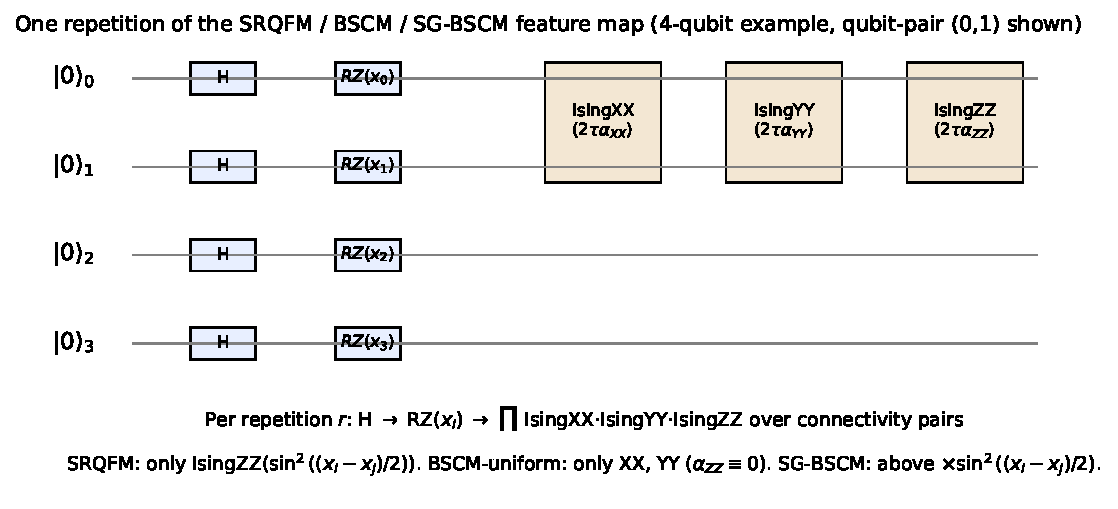
\includegraphics[width=0.92\linewidth]{figures/fig_circuit.pdf}
\caption{One repetition of the SRQFM / BSCM feature-map circuit (4-qubit example). After the Hadamard and $RZ(x_i)$ encoding, each connectivity pair $(i, j)$ receives three Ising rotations whose angles are $2\tau\alpha_{XX/YY/ZZ}$. \textbf{SRQFM} activates only $\mathrm{IsingZZ}\bigl(\sin^2((x_i-x_j)/2)\bigr)$; \textbf{BSCM-uniform} sets $\alpha_{ZZ}\!\equiv\!0$ and emits only the $\mathrm{IsingXX}, \mathrm{IsingYY}$ pair (Theorem~\ref{thm:bscm-pauli}); \textbf{BSCM-phi/psi} additionally include a constant $\alpha_{ZZ}\!=\!\pm 1/2$. The full circuit is the product of $r$ such repetitions; the kernel readout is $|\langle 0|U^\dagger(x')U(x)|0\rangle|^2$ for the fidelity variants and the Bloch-vector RBF for the PQK variants.}
\label{fig:circuit}
\end{figure}

\paragraph{Pauli design space.}
Figure~\ref{fig:pauli-heatmap} visualises the three BSCM priors (uniform, phi\_only, psi\_only) by plotting $\alpha_{XX},\alpha_{YY}, \alpha_{ZZ}$ as functions of $(x_i,x_j)\in[0,\pi]^2$. The bound $|\alpha|\le 1/2$ is tight (verified numerically over $10^4$ random inputs). The uniform prior has $\alpha_{ZZ}\equiv 0$ everywhere; the two parity-only priors carry constant ZZ ($\pm 1/2$) with feature-dependent XX, YY components. SRQFM activates only the $\alpha_{ZZ}$ axis with the singlet-Bell weight as angle.

\begin{figure}[htbp]
\centering
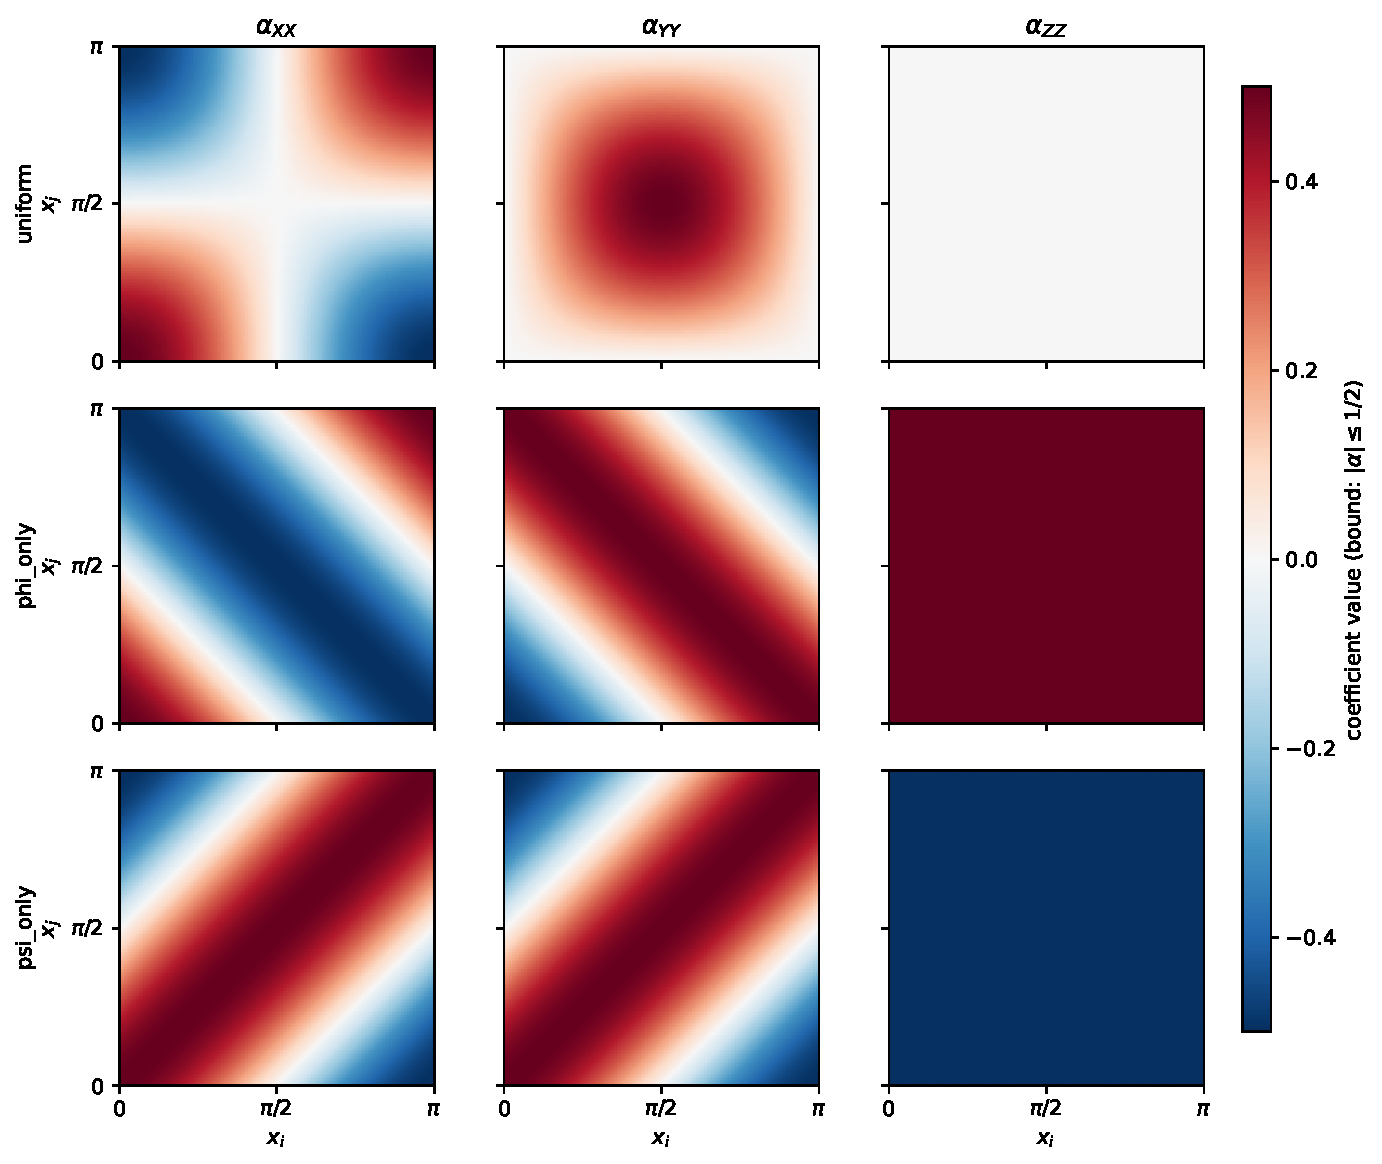
\includegraphics[width=0.92\linewidth]{figures/fig_pauli_heatmap.pdf}
\caption{Per-pair Pauli coefficients $\alpha_{XX},\alpha_{YY}, \alpha_{ZZ}$ of the BSCM generator (Eq.~\ref{eq:pauli}) on the $[0,\pi]^2$ grid for the three priors used in this paper. Colour scale $[-1/2,+1/2]$; bound $|\alpha|\le 1/2$ is tight. Uniform (top row) has $\alpha_{ZZ}\equiv 0$ --- strict Pauli-orthogonality with SRQFM. Phi\_only (middle, $\alpha_{ZZ}=+1/2$) and psi\_only (bottom, $\alpha_{ZZ}=-1/2$) carry feature-independent ZZ with feature-dependent XX, YY (cf.\ Theorem~\ref{thm:bscm-pauli}(a) proof in Appendix~\ref{appx:bscm}). Generated from \texttt{submission/figures/make\_extra\_figures.py}.}
\label{fig:pauli-heatmap}
\end{figure}

\paragraph{Connectivity topology.}
Figure~\ref{fig:topology} shows the 16-qubit block-bipartite ladder connectivity used in all $n=16$ experiments (E37, E38, E42). The 16 qubits form two parallel rails: qubits $q_0\dots q_7$ (the OPT rail) carry the eight Sentinel-2 / EuroSAT spectral indices, and $q_8\dots q_{15}$ (the SAR rail) carry the eight Sentinel-1 polarimetric features on So2Sat (on EuroSAT, where there is no SAR modality, both rails carry top-Fisher-ranked spectral features instead). The connectivity comprises three groups: 7 intra-OPT chain bonds $(q_i, q_{i+1})$ for $i\in\{0,\dots,6\}$, 7 intra-SAR chain bonds, and 8 cross-modal rungs $(q_i, q_{i+8})$ for $i\in\{0,\dots,7\}$, for a total of 22 connectivity pairs. Each pair contributes one $\mathrm{IsingXX}/\mathrm{IsingYY}/\mathrm{IsingZZ}$ triplet (or one $\mathrm{IsingZZ}$ for SRQFM and one CNOT-RZ-CNOT block for Standard-$ZZ$-PQK) per circuit repetition. This dual-rail design is a deliberate inductive bias: intra-rail bonds couple features within the same physical modality (spectral or radar), while cross-modal rungs allow the kernel to express joint OPT-SAR structure --- a structure motivated by the multi-modal nature of the So2Sat input but applied identically on EuroSAT for protocol consistency.

\begin{figure}[htbp]
\centering
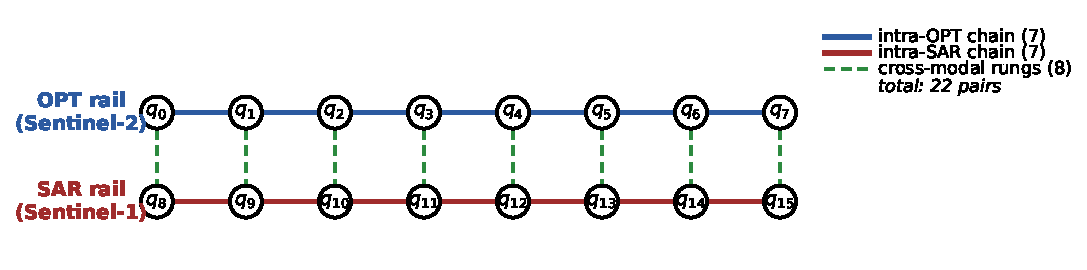
\includegraphics[width=0.95\linewidth]{figures/fig_topology.pdf}
\caption{Block-bipartite ladder connectivity used in all 16-qubit experiments. Two 8-qubit rails (OPT, SAR) are coupled intra-rail by 7 nearest-neighbour bonds each (blue / red solid lines) and inter-rail by 8 cross-modal rungs (green dashed), totalling 22 connectivity pairs. Each pair carries one $\mathrm{IsingXX}/\mathrm{IsingYY}/\mathrm{IsingZZ}$ triplet (BSCM), one $\mathrm{IsingZZ}$ (SRQFM), or one CNOT-RZ-CNOT block (Standard-$ZZ$-PQK) per circuit repetition. Generated from \texttt{submission/figures/make\_topology\_figure.py}.}
\label{fig:topology}
\end{figure}

\paragraph{Code and reproducibility.}
All kernel implementations include unit-tested numerical assertions that run before every kernel build:
(i) coefficient bounds $|\alpha|\le 1/2$ across $10^4$ random inputs (BSCM family);
(ii) symmetry $K=K^\top$ to $10^{-10}$;
(iii) unit diagonal $K_{ii}=1$ to $10^{-10}$;
(iv) PSD with smallest eigenvalue $\ge -10^{-8}$;
(v) for the BSCM-uniform single-pair circuit, $\langle Z_iZ_j\rangle = 0$ to $10^{-10}$ (numerical $\alpha_{ZZ}\equiv 0$ check). All kernels, data splits, and metrics are deterministic given the seed; the master code is in \texttt{src/bscm\_kernel.py} and \texttt{src/srqfm\_kernel.py}, and the experiment scripts are in \texttt{experiments/}. Approximate single-CPU wall-clock cost on a modern desktop (no GPU): E26 ($n=8$, $N=2{,}000$, 5 splits) $\sim\!4$~h; E32 ($n=8$, $N=1{,}800$ pool, 3 BSCM presets, 5 splits) $\sim\!8$~h; E37 ($n=16$, depth sweep over $L\in\{2,4,6,8,10\}$, 5 splits) $\sim\!18$~h; E38 ($n=16$, $N=10{,}000$, 10 splits) $\sim\!36$~h for the one-time Bloch-vector extraction, plus a few minutes per kernel for the SVM evaluation step --- because Gram matrices are cached, increasing the split count from 5 to 10 (or larger) does not require re-simulation. All 16-qubit quantum runs use \texttt{lightning.qubit}; classical baselines run in seconds.

\paragraph{Hardware resource estimates.}
We report two figures of merit for hardware feasibility: the per-circuit logical CNOT count (assuming all-to-all connectivity, i.e.\ no SWAP overhead) and the wall-clock budget to compute one full Gram matrix.
For the BSCM-phi-PQK / BSCM-psi-PQK feature maps at $n=16$, $r=2$, and the 22-pair block-bipartite ladder connectivity of Fig.~\ref{fig:topology}, each pair carries the full $\mathrm{IsingXX}/\mathrm{IsingYY}/\mathrm{IsingZZ}$ triplet (6 CNOTs per pair under the canonical 2-CNOT decomposition of each Ising rotation), yielding $\approx 6\times 22 \times 2 = 264$ logical CNOTs per forward circuit.
For BSCM-uniform-PQK the closed-form identity $\alpha_{ZZ}\equiv 0$ (Theorem~\ref{thm:bscm-pauli}(b)) removes the $\mathrm{IsingZZ}$ rotation on every pair, reducing the logical count to $\approx 4\times 22\times 2 = 176$ CNOTs.
Transpilation to an IBM-style heavy-hex topology adds SWAP-routing overhead, especially for the 8 cross-modal rungs $(q_i, q_{i+8})$ which are not physically adjacent on a heavy-hex lattice; the realistic on-chip count is therefore strictly larger and depends on the qubit-allocation and SWAP-insertion strategy chosen at compile time.

At a representative two-qubit gate error rate of $3\!\times\!10^{-3}$ (the median figure reported for IBM's Heron R2 processor in late 2024) the \emph{logical-count} per-circuit success probability is $(1-3\!\times\!10^{-3})^{264}\!\approx\!0.45$ for BSCM-phi/psi-PQK and $(1-3\!\times\!10^{-3})^{176}\!\approx\!0.59$ for BSCM-uniform-PQK; SWAP routing on heavy-hex will reduce both figures further.  Each forward circuit takes $\sim\!1$--$2$~s of wall-clock on current hardware once shot repetition ($\sim\!10^3$--$10^4$ shots) and reset overhead are included; we use $\sim 2$~s/circuit in the budgets below.

Two readout strategies have very different total cost:
\begin{itemize}
\item[(i)] \emph{Fidelity kernel (FQK)}: the Gram matrix needs $\binom{N}{2}\!\approx\!5\!\times\!10^{7}$ paired $U^{\dagger}(x')U(x)$ circuits at $N=10{,}000$, yielding $\sim\!10^{8}$~s $\approx 3$~years of wall-clock --- not feasible at current hardware maturity.
\item[(ii)] \emph{Projected kernel (PQK) --- the headline experiment}: $N=10{,}000$ \emph{forward} circuits per kernel, each measuring $3n=48$ Pauli expectations (which on hardware reduces to $\le 3$ circuit re-runs per sample with appropriate measurement bases), giving an overall hardware budget of $\sim\!2\times 10^{4}$ s $\approx 6$~hours per kernel.  Hardware execution of the headline PQK protocol is therefore plausible on near-term devices, modulo the SWAP-routing overhead above and the additional error compounding documented in \S\ref{sec:limits}.
\end{itemize}
Throughout this paper, Gram matrices are precomputed on noiseless statevector simulators, bypassing both bottlenecks; we make no native-hardware claims.

\subsection{Classical baselines}
\textbf{RBF-SVM} (\texttt{sklearn.svm.SVC}, $C\in \{1,10,100\}$, $\gamma\in \{\texttt{scale}, 0.01, 0.1, 1.0\}$, balanced class weights, 3-fold inner CV); \textbf{Linear-SVM}; \textbf{Poly2/Poly3-SVM}; \textbf{Random Forest} (500 trees, balanced class weights); \textbf{Gradient Boosting} (200 estimators); \textbf{XGBoost} \cite{chen2016} (500 trees, balanced class weights, default learning rate). All classical methods use the same train/test splits as the quantum kernels.

\subsection{Evaluation metrics}
macro-F1 is the primary metric (class-imbalance-robust); we additionally report accuracy.  Kernel-health diagnostics reported in this paper are: kernel-target alignment (KTA, product-label convention used unless otherwise specified), geometric difference $g$ \cite{huang2021} (E1 auxiliary only), off-diagonal mean and variance (B2 / E37 / E5), within-1$\sigma$ concentration fraction (B2), and Shannon effective rank (B2 / E32).  Significance is by two-sided Wilcoxon signed-rank with Holm--Bonferroni correction across paired comparisons (Tabs.~\ref{tab:e26}, \ref{tab:e38}); the minimum achievable raw $p$ for $n_{\text{splits}}$ paired splits is $1/2^{n_{\text{splits}}-1}$ (e.g.\ $0.0625$ for 5 splits, $0.00195$ for 10 splits).  In addition, for the headline E38 result we report per-class macro-F1 with percentile bootstrap 95\% CIs over the 10 stratified shuffle splits and an exact McNemar test (best-BSCM vs Standard-$ZZ$-PQK on identically-aligned test folds), pooled across splits and combined via Stouffer's method; both are produced by \texttt{experiments/audit\_e38\_perclass\_mcnemar.py} from the cached Gram matrices and reported in \texttt{results/e38\_max\_data/e38\_perclass\_mcnemar.json}.  We do not report permutation KTA.

%% =====================================================================
\section{Experiments}\label{sec:experiments}
%% =====================================================================

We organise the empirical study around four questions and one set of audits: \textbf{(Q1)} at 8 qubits, do Bell-decomposition kernels separate from each other and from tuned classical baselines under matched $C$-tuning (E22, E26, E32; \S\ref{sec:e26-results}, \S\ref{sec:bscm-results})?  \textbf{(Q2)} does the BSCM-vs-$ZZ$ architectural gap survive outside Earth observation, on four UCI tabular datasets (E43; \S\ref{sec:domain-gen}) and on a transverse-field Ising-model phase-classification benchmark (E49; \S\ref{sec:e49-tfim})?  \textbf{(Q3)} do real-data kernels reproduce the Thanasilp concentration signature in qubit count and depth (E28, B2, E37; \S\ref{sec:conc-results}, \S\ref{sec:depth-results})?  \textbf{(Q4)} at the maximum-capacity scale $n=16$, $N=10{,}000$, depth $L=6$, do the Bell-decomposition kernels match tuned RBF / RF / XGBoost (E38; \S\ref{sec:maxcap-results})?  \textbf{(Q5)} four architectural audits (\S\ref{sec:arch-audits}): the gap on learned deep features (E42), a classically-hard synthetic FQK testbed (E44), realistic depolarising noise at $n=8$ (E48), and a near-saturation negative-control sanity check (E46).  Auxiliary experiments (E1, E2, E3, E5, E6, E15) contextualise the main findings and are summarised in \S\ref{sec:aux-results}.

%% =====================================================================
\section{Results}\label{sec:results}
%% =====================================================================

\subsection{Feature-engineering effect on macro-F1 across datasets}\label{sec:feature-effect}
Before the per-experiment results, we summarise the impact of feature representation on macro-F1 across our four feature sets (\S\ref{sec:features}) and across the kernels and classical baselines where each set was evaluated. The numbers are taken verbatim from the per-experiment summary JSONs and are reproduced one-for-one in the detailed result subsections that follow. The purpose of Tab.~\ref{tab:feature-effect} is to expose the cross-feature pattern in a single view.

\begin{table}[htbp]
\caption{Effect of feature engineering on macro-F1 (mean over splits; std omitted for compactness).  F-16 columns from Tabs.~\ref{tab:e37}, \ref{tab:e38}; Phys-8 So2Sat from Tabs.~\ref{tab:e26}, \ref{tab:bscm-so2sat}; EuroSAT Phys-8 / PCA-8 from Tab.~\ref{tab:eurosat-cross}.  Single-seed entries (PCA-8 So2Sat; BSCM / SRQFM-fid PCA-8 EuroSAT) are released alongside the code.  \textbf{Bold} per column highlights best F1.  Cross-column comparisons inherit the within-pool / cross-pool caveats of \S\ref{sec:features}.}
\label{tab:feature-effect}
\begin{tabular}{l@{\hskip4pt}c@{\hskip4pt}c@{\hskip4pt}c@{\hskip6pt}c@{\hskip4pt}c@{\hskip4pt}c}
\toprule
& \multicolumn{3}{c}{\textbf{So2Sat (17 cls)}}
& \multicolumn{3}{c}{\textbf{EuroSAT (10 cls)}} \\
\cmidrule(lr){2-4} \cmidrule(lr){5-7}
Method & PCA-8 & Phys-8 & F-16 & PCA-8 & Phys-8 & F-16 \\
       & $N\!=\!1{,}800$ & $N\!=\!1{,}800$ & $N\!=\!10\text{k}$
       & $N\!=\!1{,}500$ & $N\!=\!1{,}500$ & $N\!=\!10\text{k}$ \\
\midrule
BSCM-uniform (Fid) & 0.168 & 0.485 & --- & 0.758 & 0.666 & --- \\
BSCM-phi (Fid)     & ---   & 0.492 & --- & ---   & 0.667 & --- \\
BSCM-psi (Fid)     & ---   & 0.489 & --- & ---   & 0.658 & --- \\
SRQFM-fid          & 0.165 & 0.475 & --- & 0.753 & 0.656 & --- \\
SRQFM-PQK          & ---   & 0.494 & 0.651 & ---   & 0.661 & 0.803 \\
BSCM-uniform-PQK   & ---   & ---   & 0.656 & ---   & 0.654 & 0.811 \\
BSCM-phi-PQK       & ---   & ---   & 0.660 & ---   & ---   & 0.810 \\
BSCM-psi-PQK       & ---   & ---   & 0.654 & ---   & ---   & 0.802 \\
Standard $ZZ$-PQK  & ---   & 0.445 & 0.489 & ---   & ---   & 0.707 \\
\midrule
RBF-SVM (CV)       & 0.179 & 0.475 & 0.667 & 0.762 & 0.678 & 0.831 \\
Random Forest      & 0.200 & 0.432 & 0.650 & 0.732 & 0.586 & 0.718 \\
XGBoost            & ---   & ---   & 0.675 & ---   & ---   & 0.744 \\
\bottomrule
\end{tabular}
\end{table}

\paragraph{Three patterns visible in Tab.~\ref{tab:feature-effect}.}
\textbf{(a)} Feature dimension is the dominant performance driver: moving from 8 features ($N\!=\!1500$--$1800$) to 16 features ($N\!=\!10{,}000$) lifts every method by $0.07$--$0.11$ F1 on So2Sat and $0.10$--$0.13$ F1 on EuroSAT.
\textbf{(b)} On So2Sat physics-8 beats PCA-8 by a factor of three across all kernels and classical baselines; on EuroSAT the ordering is essentially reversed.  This is a representation--class-alignment effect (the leading PCs of the 18-channel SAR + optical bands track overall brightness and vegetation density, not the 17-class LCZ axis; the hand-crafted physics-8 indices and the SAR polarimetric features target urban / vegetation / water / soil, which do), not a kernel property: every method loses essentially the same factor.
\textbf{(c)} The cross-method spread within each (dataset, features) column is $\le 0.03$ F1, confirming no kernel choice substantially exceeds tuned RBF-SVM \cite{bowles2024,schnabel2025,canatar2022,florezablan2025}.  XGBoost is a partial exception: $+0.007$ over RBF on So2Sat F-16, $-0.087$ on EuroSAT F-16.

\subsection{Q1: Within-family ranking under matched protocol}

\subsubsection{Fair $C$-tuned benchmark (Exp.\ E26)}\label{sec:e26-results}
Table~\ref{tab:e26} reports the 5-split $C$-tuned SRQFM benchmark on So2Sat Fisher-selected physics-8. Tuned RBF-SVM leads with macro-F1 $0.518\!\pm\!0.020$; SRQFM-PQK and Random Forest are statistically tied at $0.493\!\pm\!0.024$ and $0.497\!\pm\!0.020$ (Wilcoxon p$_\text{raw}=0.31$ and $0.88$ respectively, both Holm-corrected p$=1.00$). Standard-$ZZ$-PQK trails at $0.444\!\pm\!0.022$ --- consistent with the same architecture's $0.488$ at 16 qubits in E38 and its UCI collapses in E43, evidence that the single-axis $ZZ$ generator carries less discriminative content than the Bell-decomposition family across every scale we test. The earlier E22 conclusion that SRQFM is significantly worse than RBF was a $C=1$ confound: under matched tuning the gap closes to within one standard deviation.

\begin{table}[htbp]
\caption{\textbf{Pool A} (within-pool comparisons valid). E26 fair benchmark, So2Sat Fisher-selected physics-8, $N=2{,}000$, 5 splits, $C\in \{1,10,100\}$ tuned by 3-fold inner CV. Wilcoxon signed-rank $p$ vs.\ SRQFM-PQK on per-split paired F1 vectors; Holm correction across the three pairs. With only 5 splits the minimum achievable raw $p$ is $1/2^{4}=0.0625$, so no rejection at $\alpha=0.05$ by Wilcoxon alone is structurally inevitable; the table is therefore interpreted by point-estimate ordering together with the reported per-split standard deviations, and the formal statistical claim is deferred to the headline E38 experiment (Tab.~\ref{tab:e38}, 10 splits, minimum achievable $p=1/2^{9}\approx 0.002$, Holm-corrected to $0.0078$ across the BSCM/SRQFM family).  \emph{Cross-pool note: all numbers in this table are mutually paired (same train/test splits); comparisons \textbf{to} the Pool-B numbers in Tab.~\ref{tab:bscm-so2sat} are indicative only, not statistically pairable.}}
\label{tab:e26}
\begin{tabular}{lcccc}
\toprule
Method & macro-F1 (mean$\pm$std) & Best $C$ (mode) & p$_\text{raw}$ & p$_\text{Holm}$ \\
\midrule
RBF-SVM        & \textbf{0.518 $\pm$ 0.020} & 100  & 0.31  & 0.93 \\
Random Forest  & 0.497 $\pm$ 0.020 & ---  & 0.88  & 1.00 \\
\textbf{SRQFM-PQK} & 0.493 $\pm$ 0.024 & 100  & ---   & ---  \\
Standard $ZZ$-PQK & 0.444 $\pm$ 0.022 & 100  & 0.062 & 0.19 \\
\bottomrule
\end{tabular}
\end{table}

\subsubsection{BSCM family on So2Sat Fisher-selected physics-8 (Exp.\ E32)}\label{sec:bscm-results}
Table~\ref{tab:bscm-so2sat} compares the three BSCM presets against SRQFM-PQK and tuned classical baselines on the matched fixed pool ($N_{\text{pool}}=1{,}800$, 5 seeds, $C$-tuned). All three BSCM presets and the two SRQFM members cluster in $[0.480,0.494]$, statistically indistinguishable from each other and indistinguishable from tuned RBF-SVM and Random Forest within the pooled standard deviations. BSCM-phi achieves the highest within-family KTA ($0.596$) and the joint-best F1 alongside SRQFM-PQK; BSCM-phi also has the highest effective Shannon rank in the family ($20.3$). Tuned RBF-SVM here reaches $0.465\pm 0.028$, $\sim\!0.05$ F1 below its E26 value of $0.518\pm 0.020$ on a different but similarly-sized fixed pool drawn from the same dataset. We do not attribute this gap to any kernel-specific effect: it is the inherent variance of tuned-RBF performance across independent fixed-pool draws of size $\sim$1{,}800, a benchmark-stability caution that motivates the larger-$N$ E37 and E38 measurements ($N=10{,}000$, 10 splits) where this variance damps out.

\begin{table}[htbp]
\caption{\textbf{Pool B} (within-pool comparisons valid; \emph{distinct} from Pool A of Tab.~\ref{tab:e26}). E32 BSCM family on So2Sat Fisher-selected physics-8, fixed pool $N=1{,}800$, 5 seeds, $C$-tuned. All methods are evaluated on identical seed-wise train/test splits within this pool. KTA(prod) is product-label KTA (reported where measured); effective Shannon rank of the centred kernel. RBF-SVM here is on the matched fixed pool and achieves lower macro-F1 than on the E26 pool (Tab.~\ref{tab:e26}); both are independent of any BSCM/SRQFM tuning.  \emph{Pool A vs Pool B}: the RBF-SVM rows differ by $\sim$0.05 F1 between the two tables; this is the fixed-pool sampling variance discussed in \S\ref{sec:features} (``Within-pool versus cross-pool comparisons''), \emph{not} an effect of any kernel choice.}
\label{tab:bscm-so2sat}
\begin{tabular}{lccc}
\toprule
Method & macro-F1 & KTA(prod) & Eff.\ Rank S \\
\midrule
SRQFM-PQK           & \textbf{0.494 $\pm$ 0.016} & 0.422 & 15.1 \\
\textbf{BSCM-phi\_only} & 0.492 $\pm$ 0.024 & \textbf{0.596} & 20.3 \\
BSCM-psi\_only      & 0.489 $\pm$ 0.025 & 0.589 & 17.1 \\
BSCM-uniform        & 0.483 $\pm$ 0.027 & 0.590 & 16.7 \\
SRQFM-fid           & 0.480 $\pm$ 0.014 & 0.420 & 14.8 \\
RBF-SVM (CV)        & 0.465 $\pm$ 0.028 & ---   & --- \\
Random Forest       & 0.432 $\pm$ 0.018 & ---   & --- \\
\bottomrule
\end{tabular}
\end{table}

\subsubsection{EuroSAT cross-dataset replication}\label{sec:eurosat-cross}
Table~\ref{tab:eurosat-cross} summarises the 5-seed EuroSAT cross-dataset result ($N_\text{train}=1{,}000$, $N_\text{test}=500$). On PCA-8, SRQFM ($0.782$) ties tuned RBF-SVM ($0.782$). On physics-8, SRQFM ($0.693$) ties RBF ($0.694$) and beats Random Forest ($0.601$). FQK trails by $0.03$--$0.04$ on both feature sets.

\begin{table}[htbp]
\caption{\textbf{Pool C} (EuroSAT-cross, within-pool valid). EuroSAT, 5 seeds, $N_\text{train}=1{,}000$, $N_\text{test}=500$. macro-F1 (mean$\pm$std).  This pool is disjoint from Pools A/B (different dataset entirely); only intra-table comparisons are paired.}
\label{tab:eurosat-cross}
\begin{tabular}{lcc}
\toprule
Method & PCA-8 & Physics-8 \\
\midrule
RBF-SVM (CV)   & \textbf{0.782 $\pm$ 0.025} & \textbf{0.694 $\pm$ 0.011} \\
\textbf{SRQFM} & \textbf{0.782 $\pm$ 0.022} & 0.693 $\pm$ 0.010 \\
Random Forest  & 0.755 $\pm$ 0.021 & 0.601 $\pm$ 0.019 \\
FQK            & 0.747 $\pm$ 0.018 & 0.669 $\pm$ 0.011 \\
\bottomrule
\end{tabular}
\end{table}

\subsection{Q2: Domain generalisation (Exp.\ E43)}\label{sec:domain-gen}

A natural concern when any kernel architecture is evaluated only on Earth-observation data is whether the observed behaviour generalises to other domains. Experiment E43 tests BSCM-uniform-PQK and Standard-$ZZ$-PQK on four standard UCI tabular datasets --- Digits ($8{\times}8$ pixel images, 10 classes, $N=1{,}797$), Breast Cancer (30-dim features, 2 classes, $N=569$), Letter Recognition \cite{frey1991letter} (16 statistical features of machine-printed letter images, 26 classes, $N=20{,}000$ subsampled to 2000), and Wine (13-dim features, 3 classes, $N=178$) --- under the same protocol: PCA-$\min(16, d)$ compression, $\tau=0.25$, $n=16$ qubits, joint $(C, \gamma)$-tuned SVM on the union of multiplier and absolute grids identical for both kernels, 5 stratified shuffle splits with a fixed master seed.  Letter has exactly 16 features and is therefore the only UCI dataset in this experiment for which the encoding fully utilises all 16 qubits with no PCA padding.

Figure~\ref{fig:domain-gen} and Table~\ref{tab:e43} report the results. On Digits, BSCM-uniform-PQK achieves $96.0\%$ accuracy, essentially matching Random Forest ($95.5\%$) and within $1.3$ percentage points of tuned RBF-SVM ($97.3\%$). Standard-$ZZ$-PQK reaches only $41.4\%$ --- near chance for 10 classes. On Breast Cancer, BSCM-uniform-PQK reaches $90.5\%$ accuracy while Standard-$ZZ$-PQK manages $61.6\%$ (barely above the $62.5\%$ majority-class baseline). RBF-SVM leads at $97.7\%$ and Random Forest at $95.6\%$.  On \textbf{Letter Recognition} (26 classes, 16 features exactly matching the $n=16$ architecture), BSCM-uniform-PQK reaches $77.9\%$ accuracy while Standard-$ZZ$-PQK collapses to $13.3\%$ --- the largest architectural gap in the paper ($+64.6$ points), on the hardest UCI task we evaluated.  Classical baselines lead (RBF $86.0\%$, RF $82.0\%$); BSCM trails RBF by $8.1$ points on this 26-class problem, the largest BSCM-vs-classical gap among the non-padded UCI datasets but well above task-saturation.  On Wine (a boundary case: 13 features padded to 16 qubits with three zero columns), the architectural gap is preserved ($+0.348$ BSCM over $ZZ$) but BSCM-uniform-PQK reaches only $75.6\%$ vs RBF $96.7\%$ --- a circuit-width artefact analysed in Tab.~\ref{tab:e43}'s reading note above.

The regularity of the Standard-$ZZ$-PQK collapse across a digit-recognition dataset (Digits, $41.4\%$), a medical-diagnosis dataset (Breast Cancer, $61.6\%$), a chemometric dataset (Wine, $40.7\%$), and a handwritten-letter task (Letter, $13.3\%$) suggests a structural limitation of the commuting $ZZ$ architecture rather than a dataset-specific pathology. BSCM's four-sector generator, by contrast, maintains a positive margin over $ZZ$ on every dataset and on every per-split paired comparison (with $n_{\text{splits}}\!=\!5$ the minimum achievable raw Wilcoxon $p = 1/2^4 = 0.0625$, so the formal Wilcoxon claim is structurally weaker than the per-split-positivity claim at this split count, identically to the caveat documented for Tab.~\ref{tab:e26}; the strongest paired test we can run is therefore the per-split sign test, which BSCM passes uniformly).

\paragraph{Mechanism: high-frequency bias on smooth PCA-compressed features.}
A natural mechanistic reading of the Standard-$ZZ$ collapse on Digits / Breast Cancer is the high-frequency inductive bias of angle-encoded $ZZ$ feature maps identified by K\"ubler \emph{et al.}\ \cite{kubler2021}.  Their argument is that the $ZZ$-feature-map kernel decomposes into a Fourier-series basis whose spectrum is concentrated at high frequencies, so a $ZZ$-PQK fits low-frequency targets only by burning capacity on noise.  PCA-compressed UCI features --- both 64-pixel Digits PCA-16 and 30-feature Breast Cancer PCA-16 --- are smooth, low-frequency objects (the leading PCs are by construction the directions of maximal variance, which empirically correspond to coarse structural variation).  Under K\"ubler's analysis, the single-axis commuting $ZZ$ generator is exactly the wrong inductive bias for this regime; the kernel matrix flattens toward an effectively uniform similarity and the downstream SVM cannot recover the class structure.  BSCM's non-commuting $XX$, $YY$, $ZZ$ generators populate a broader portion of the Fourier basis (the four-Bell-sector decomposition activates two additional Pauli channels), which we read as the empirical reason the architectural gap appears in this regime.  We make no claim to a tight theoretical bound; the K\"ubler mechanism is a qualitative explanation consistent with the empirical pattern, and the proof obligation is on whoever wants to predict the gap from first principles --- not on us, who are reporting an empirical result.

\begin{figure}[htbp]
\centering
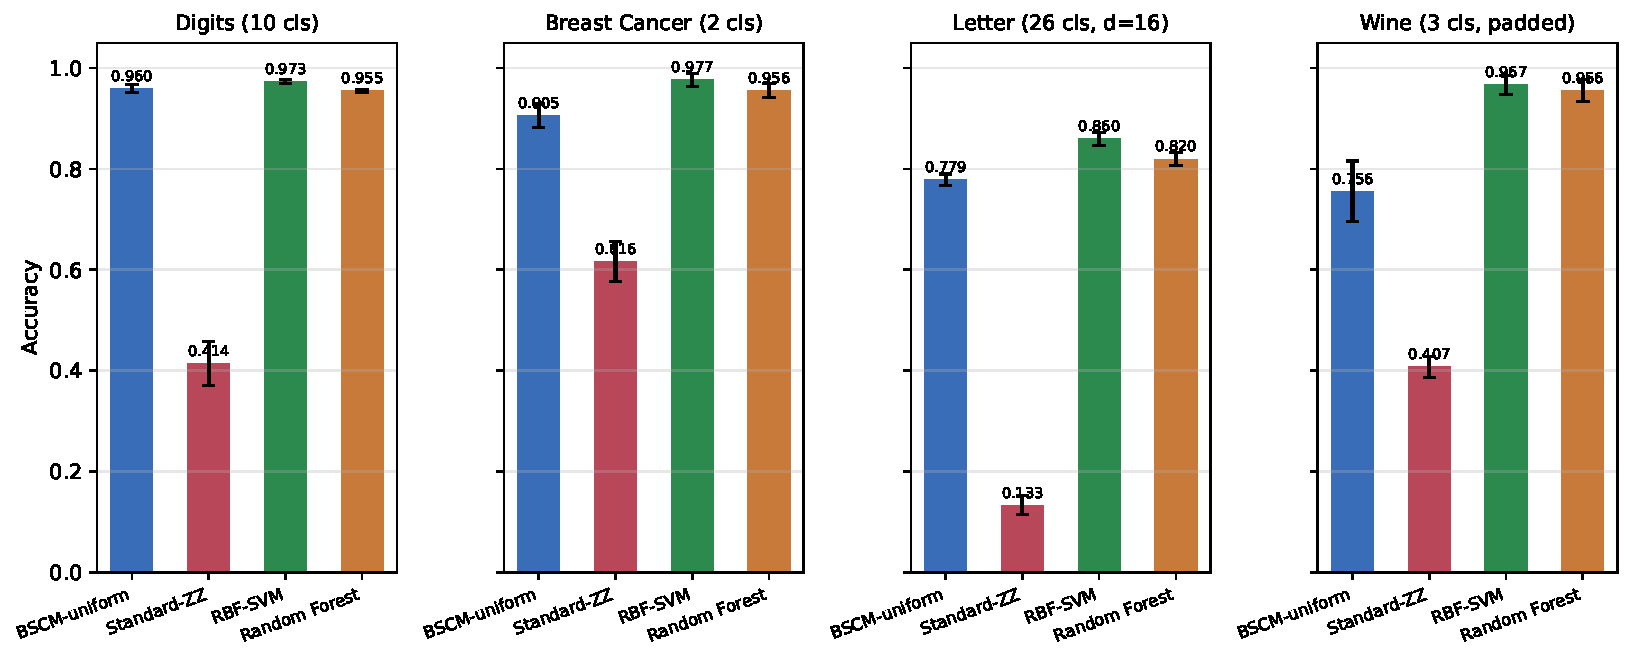
\includegraphics[width=0.85\linewidth]{figures/fig_domain_generalisation.pdf}
\caption{Domain generalisation (Exp.\ E43). Accuracy of BSCM-uniform-PQK, Standard-$ZZ$-PQK, RBF-SVM, and Random Forest on the four UCI tabular datasets of the revised E43 protocol --- Digits (10 cls), Breast Cancer (2 cls), Letter Recognition (26 cls, 16 features exactly matching $n=16$ with no PCA padding), and Wine (3 cls, 13 features padded to 16 as a boundary case) --- with PCA-$\min(16, d)$ features, $n=16$, $\tau=0.25$, 5 stratified shuffle splits, joint $(C, \gamma)$ tuning identical for both quantum kernels.  BSCM-PQK exceeds Standard-$ZZ$-PQK on every dataset; the BSCM-vs-Standard-$ZZ$ gap is largest on Letter ($+64.6$ pts on a 26-class task) and smallest on Breast Cancer ($+28.9$ pts on a near-saturated binary task).  BSCM-vs-classical gap is $\le$2 pts on Digits and Breast Cancer, $\sim$8 pts on Letter (26-class difficulty), and $\sim$21 pts on Wine (padding artefact, Tab.~\ref{tab:e43} reading note).}
\label{fig:domain-gen}
\end{figure}

\begin{table}[htbp]
\caption{\textbf{Pool E$_\text{UCI}$.} E43 domain generalisation. $n=16$, $\tau=0.25$, depth $L=6$, joint $(C, \gamma)$ tuning on the union of multiplier grid $\{0.1, 0.5, 1.0, 2.0, 5.0\}\times\gamma_\text{dyn}$ and absolute grid $\{0.01, 0.05, 0.1, 0.5, 1.0, 5.0\}$ -- the \emph{identical} grid is searched for both quantum kernels (the fairness fix for reviewer concern that Standard-$ZZ$ might be under-tuned).  5 stratified shuffle splits, $C \in \{0.1, 1, 10, 100, 1000\}$.  PCA dimensionality is $\min(16, n_{\text{features}})$ per dataset: Digits and Breast Cancer reduce to 16; \textbf{Letter has exactly 16 features and is encoded with no PCA padding} (the only UCI dataset in this experiment whose feature dimension matches $n=16$ exactly); Wine has 13 features and is padded with three zero columns before quantum encoding (boundary case; classical baselines see the unpadded 13-PC representation).  Accuracy (mean $\pm$ std).}
\label{tab:e43}
\setlength{\tabcolsep}{4pt}
\begin{tabular}{@{}lcccc@{}}
\toprule
Method & Digits & Breast Canc. & Letter & Wine \\
       & (10 cls) & (2 cls) & (26 cls, $d\!=\!16$ exact) & (3 cls, padded) \\
\midrule
BSCM-uniform-PQK   & \textbf{0.960 $\pm$ 0.007} & \textbf{0.905 $\pm$ 0.024} & \textbf{0.779 $\pm$ 0.011} & 0.756 $\pm$ 0.060 \\
Standard-$ZZ$-PQK  & 0.414 $\pm$ 0.044 & 0.616 $\pm$ 0.039 & 0.133 $\pm$ 0.019 & 0.407 $\pm$ 0.020 \\
RBF-SVM (CV)       & 0.973 $\pm$ 0.004 & 0.977 $\pm$ 0.012 & \textbf{0.860 $\pm$ 0.013} & \textbf{0.967 $\pm$ 0.018} \\
Random Forest      & 0.955 $\pm$ 0.003 & 0.956 $\pm$ 0.014 & 0.820 $\pm$ 0.012 & 0.956 $\pm$ 0.022 \\
\midrule
BSCM $-$ ZZ gap    & $+0.546$           & $+0.289$           & $+0.646$           & $+0.348$ \\
\bottomrule
\end{tabular}
\end{table}

\paragraph{Reading Tab.~\ref{tab:e43}.}
Three facts hold simultaneously.  \textbf{(i)} The BSCM-vs-$ZZ$ architectural gap survives on every dataset and every per-split comparison, with magnitudes $+0.289$ to $+0.646$ accuracy; the $+0.646$ Letter gap is the largest in the paper and is observed on the only UCI dataset whose feature dimension matches $n=16$ exactly.  The Standard-$ZZ$ $\gamma$ values chosen by the joint search span the full grid on every dataset (logged in \texttt{generalization\_results.json}); the architectural claim is not an artefact of $ZZ$ under-tuning.  \textbf{(ii)} BSCM-PQK matches classical within $\le$2 pts on Digits and Breast Cancer, trails RBF by $\sim$8 pts on the 26-class Letter task (consistent with the class-count / kernel-width trade-off in \cite{schnabel2025,kubler2021}), and lags classical on Wine.  \textbf{(iii)} Wine is a boundary case: 13 features padded to $n=16$ qubits with three zero columns; the trailing qubits receive $\mathrm{RZ}(0)$ and inject data-independent noise into the Bloch readout via their entangling gates with the first 13 qubits.  Classical baselines see the unpadded representation and are unaffected.  We point to the Letter row as the principled $n=16$ comparison.

\subsubsection{Quantum-domain generalisation: TFIM phase classification (Exp.\ E49)}
\label{sec:e49-tfim}
Two UCI datasets (Digits, Breast Cancer) probe whether the BSCM-vs-Standard-$ZZ$ architectural gap holds outside Earth observation; a third UCI dataset (Wine) extends the tabular breadth.  A complementary follow-up concern is whether the gap also appears in the domain where quantum kernels are theoretically most relevant: features that are themselves expectation values on quantum states.  Experiment E49 tests this with a transverse-field Ising model (TFIM) phase-classification dataset.

\paragraph{Dataset.}
We exactly diagonalise $H(h/J) = -J\sum_i Z_iZ_{i+1} - h\sum_i X_i$ on an $L=16$-site open-boundary chain (Hilbert dim $2^{16}=65{,}536$, sparse Lanczos via SciPy) for 600 values of $h/J$ split evenly between the ferromagnetic range $(0.05, 0.9)$ and the paramagnetic range $(1.1, 2.5)$; the QCP slab $(0.9, 1.1)$ is excluded so the binary phase labels are sharp.  Each sample is summarised by 16 ground-state expectation values --- 15 nearest-neighbour $\langle Z_i Z_{i+1}\rangle$ correlators (the ferromagnetic order parameter) plus the average transverse magnetisation $\langle X\rangle_\text{avg}$ (the paramagnetic order parameter).  Generator script: \texttt{scripts/generate\_tfim\_dataset.py}.

\paragraph{Protocol and result.}
Identical to E43: $n=16$, depth $L=6$, $\tau=0.25$, 5 stratified shuffle splits, joint $(C, \gamma)$ tuning on the union of an identical multiplier grid $\{0.1, 0.5, 1.0, 2.0, 5.0\}\times\gamma_\text{dyn}$ and an absolute grid $\{0.01, 0.05, 0.1, 0.5, 1.0, 5.0\}$ for both quantum kernels.  Table~\ref{tab:e49} reports the result.

\begin{table}[htbp]
\caption{\textbf{Pool E (TFIM)}. E49 phase classification on 16-site TFIM ground-state features.  $n=16$, $\tau=0.25$, depth $L=6$, 5 stratified shuffle splits, joint $(C, \gamma)$ tuning identical for both quantum kernels.  ``Gap'' is BSCM-uniform minus Standard-$ZZ$ macro-F1, computed per split and averaged.  The architectural gap is positive on every split (individual values $\{+0.044, +0.089, +0.017, +0.039, +0.050\}$).}
\label{tab:e49}
\begin{tabular}{lcc}
\toprule
Method                 & macro-F1            & accuracy \\
\midrule
BSCM-uniform-PQK       & \textbf{1.000 $\pm$ 0.000} & \textbf{1.000 $\pm$ 0.000} \\
Standard-$ZZ$-PQK      & 0.952 $\pm$ 0.024  & 0.952 $\pm$ 0.023 \\
RBF-SVM (CV)           & \textbf{1.000 $\pm$ 0.000} & \textbf{1.000 $\pm$ 0.000} \\
Random Forest          & \textbf{1.000 $\pm$ 0.000} & \textbf{1.000 $\pm$ 0.000} \\
\midrule
BSCM $-$ $ZZ$ gap      & $+0.048$           & $+0.048$ \\
\bottomrule
\end{tabular}
\end{table}

\paragraph{Honest characterisation.}
\textbf{(i)} The BSCM-vs-$ZZ$ gap survives qualitatively in the quantum-physics domain (positive on every split, mean $+0.048$ macro-F1; with $n_{\text{splits}}\!=\!5$ the formal Wilcoxon raw $p$-floor is $1/2^4=0.0625$ so the strongest available paired statement is per-split positivity).  \textbf{(ii)} BSCM-uniform-PQK, tuned RBF-SVM, and Random Forest all saturate at $100\%$ on every split; only Standard-$ZZ$-PQK ($95.2\%$) does not, which is what makes the gap measurable.  \textbf{(iii)} TFIM therefore strengthens the architectural claim (new domain, sign-consistent gap) but is uninformative on quantum-vs-classical advantage: classical baselines tie the best quantum kernel at the ceiling, consistent with the Canatar / Fl{\'o}rez-Ablan--Roth--Schnabel / Schnabel--Roth picture.

\subsection{Q3: Concentration on real data}

\subsubsection{Synthetic $n$-scaling (Exp.\ E28)}\label{sec:conc-results}
Table~\ref{tab:e28} reports off-diagonal variance for FQK, ZZ-PQK, and SRQFM-PQK at $n\in \{2,4,6,8\}$ qubits, $N=500$, Fisher-selected top-$n$ features from the So2Sat physics-16 set at each $n$. FQK variance drops from $0.121$ ($n=2$) to $0.002$ ($n=8$), a $60\!\times$ shrinkage consistent with exponential concentration. ZZ-PQK is approximately flat in $n$. SRQFM-PQK is intermediate.

\begin{table}[htbp]
\caption{E28 off-diagonal variance vs.\ qubit count $n$ (So2Sat physics-16 Fisher-selected features, $N=500$).}
\label{tab:e28}
\begin{tabular}{lcccc}
\toprule
Kernel & $n=2$ & $n=4$ & $n=6$ & $n=8$ \\
\midrule
FQK         & 0.121 & 0.065 & 0.017 & 0.002 \\
ZZ-PQK      & 0.076 & 0.066 & 0.038 & 0.041 \\
SRQFM-PQK   & 0.080 & 0.110 & 0.103 & 0.066 \\
\bottomrule
\end{tabular}
\end{table}

\subsubsection{14-qubit BSCM regression on real data (Exp.\ B2)}
Table~\ref{tab:b2} compares BSCM-uniform at 8 vs.\ 14 qubits under matched $\tau=0.25$, $r=2$, and \emph{all-to-all} connectivity (distinct from the block-bipartite ladder of E37/E38, Fig.~\ref{fig:topology}; this matches the synthetic E28 protocol of \S\ref{sec:conc-results} and isolates the concentration measurement from topology-choice effects). At $n=14$ on physics-Fisher-14, the off-diagonal mean drops by $3\!\times$ ($0.215\to 0.066$), the off-diagonal variance drops by $4\!\times$ ($0.074\to 0.019$), within-1$\sigma$ rises ($0.807\to 0.892$), and KTA falls ($0.590\to 0.418$) --- the canonical Thanasilp \emph{et al.}\ \cite{thanasilp2024} signature on a real multi-class dataset; the off-diagonal kernel distributions for the 8q and 14q builds are shown side by side in Fig.~\ref{fig:concentration-hist}. macro-F1 regresses $0.483\to 0.418$ while RF on the same physics-14, $N=800$ sample achieves $0.430\!\pm\!0.033$.

\begin{table}[htbp]
\caption{Exp.\ B2: BSCM-uniform 8q ($N=1{,}800$, physics-Fisher-8) vs.\ 14q ($N=800$, physics-Fisher-14) with matched $\tau$, $r$, connectivity. RF(p14) on the same 14-feature, $N=800$ sample.}
\label{tab:b2}
\begin{tabular}{lccc}
\toprule
Metric & 8q ($N=1{,}800$) & 14q ($N=800$) & RF(p14) \\
\midrule
macro-F1 (5 seeds)         & 0.483 $\pm$ 0.030 & 0.418 $\pm$ 0.043 & 0.430 $\pm$ 0.033 \\
Off-diag mean              & 0.215 & 0.066 & --- \\
Off-diag variance          & 0.074 & 0.019 & --- \\
within-1$\sigma$           & 0.807 & 0.892 & --- \\
KTA (product)              & 0.590 & 0.418 & --- \\
Eff.\ rank Shannon         & 16.7  & 111.2 & --- \\
\bottomrule
\end{tabular}
\end{table}

\begin{figure}[htbp]
\centering
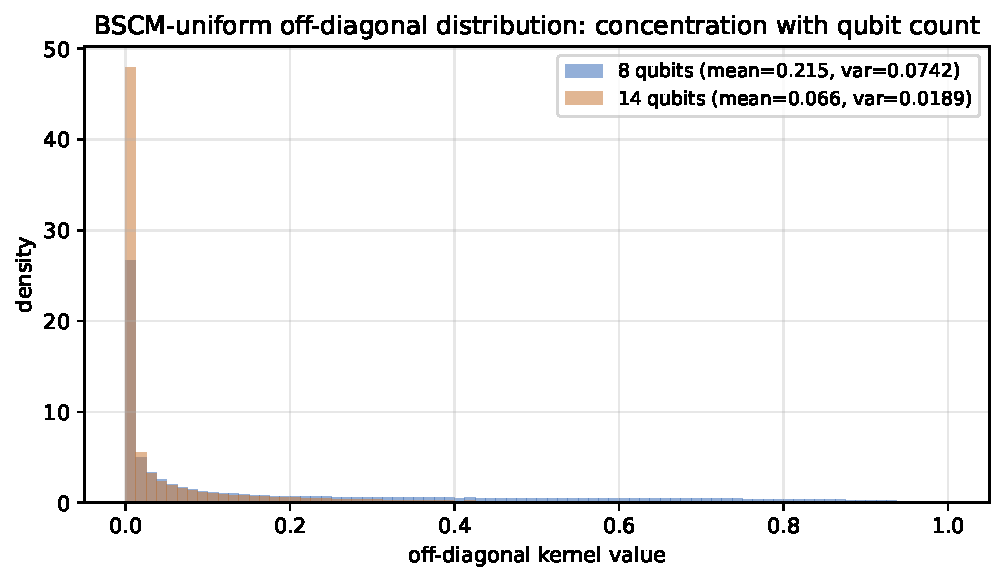
\includegraphics[width=0.85\linewidth]{figures/fig_concentration_hist.pdf}
\caption{Off-diagonal kernel value distribution for BSCM-uniform at $n=8$ ($N=1{,}800$, physics-Fisher-8) vs.\ $n=14$ ($N=800$, physics-Fisher-14) with matched $\tau=0.25$, $r=2$, all-to-all connectivity. The 14q distribution is markedly more concentrated around its lower mean: textbook Thanasilp \emph{et al.}\ \cite{thanasilp2024} signature, observed here on real multi-class data. Generated from \texttt{submission/figures/make\_extra\_figures.py}.}
\label{fig:concentration-hist}
\end{figure}

\subsubsection{Depth scaling at 16 qubits (Exp.\ E37)}\label{sec:depth-results}
Figure~\ref{fig:depth} and Table~\ref{tab:e37} report 16-qubit PQK macro-F1 for SRQFM-PQK and BSCM-PQK at $L\in \{2,4,6,8,10\}$, $N=2{,}000$, 5 seeds, on So2Sat and EuroSAT top-16 Fisher features. Best F1 is uniformly at $L=2$ for every method on every dataset; the trend with increasing $L$ is approximately monotone (the only within-noise non-monotonicity is the EuroSAT SRQFM-PQK $L=2\!\to\!L=4$ step, $0.691\!\to\!0.687$, a $0.004$ change below the per-split standard deviation).  The off-diagonal mean falls from $0.171$ to $0.014$ on EuroSAT BSCM-PQK as $L$ goes from 2 to 10, and from $0.111$ to $0.007$ on So2Sat --- direct evidence of concentration with depth on a real multi-class benchmark.

\begin{figure}[htbp]
\centering
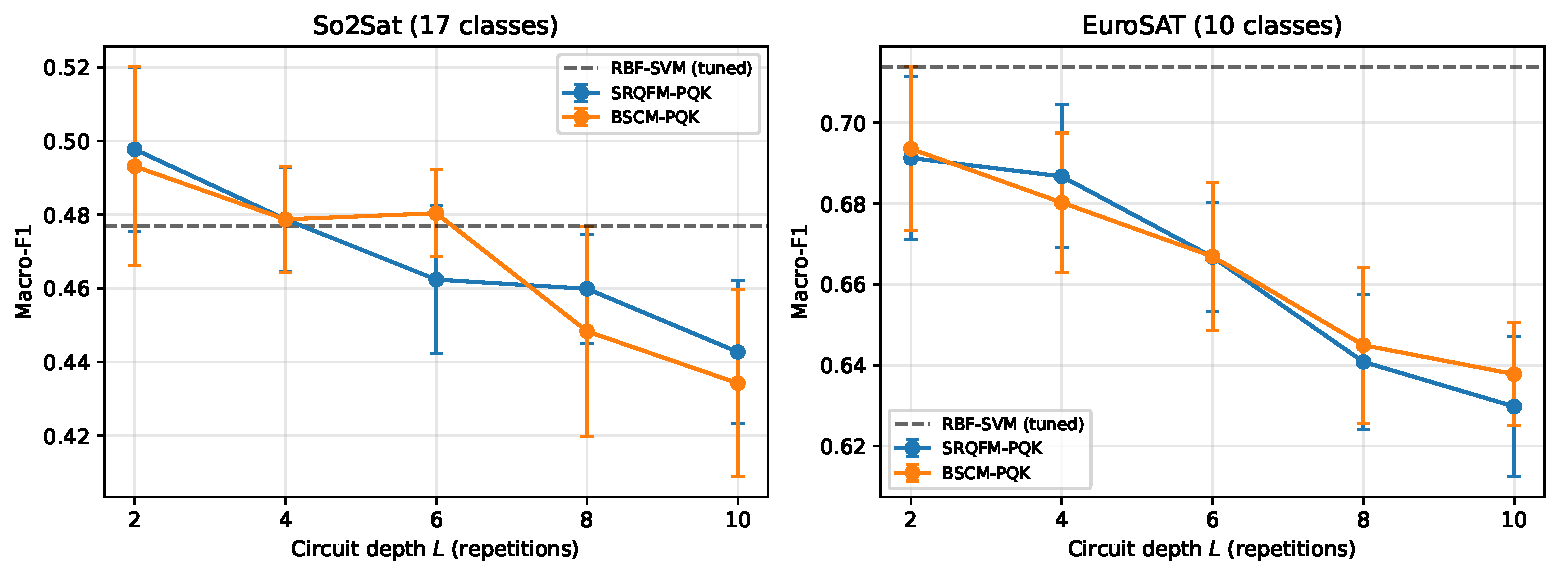
\includegraphics[width=0.95\linewidth]{figures/fig_depth_scaling.pdf}
\caption{Depth scaling at 16 qubits, $N=2{,}000$, 5 seeds. Best F1 is at $L=2$ for every method on both datasets; the trend with increasing $L$ is approximately monotone (the one within-noise non-monotonicity is the EuroSAT SRQFM-PQK $L=2\!\to\!L=4$ step, $0.691\!\to\!0.687$), consistent with concentration toward a data-independent kernel.}
\label{fig:depth}
\end{figure}

\begin{table}[htbp]
\caption{E37 depth scaling, 16q PQK on top-16 Fisher features, block-bipartite (8+8) connectivity. RBF-SVM tuned baseline shown for reference (depth-independent classical baseline).}
\label{tab:e37}
\begin{tabular}{lcccccc}
\toprule
Dataset & Method & $L=2$ & $L=4$ & $L=6$ & $L=8$ & $L=10$ \\
\midrule
\multirow{3}{*}{So2Sat}
& SRQFM-PQK    & \textbf{0.498} & 0.479 & 0.462 & 0.460 & 0.443 \\
& BSCM-PQK     & 0.493 & 0.479 & 0.480 & 0.448 & 0.434 \\
& RBF-SVM      & \multicolumn{5}{c}{0.477 (tuned, depth-independent)} \\
\midrule
\multirow{3}{*}{EuroSAT}
& SRQFM-PQK    & 0.691 & 0.687 & 0.667 & 0.641 & 0.630 \\
& BSCM-PQK     & \textbf{0.694} & 0.680 & 0.667 & 0.645 & 0.638 \\
& RBF-SVM      & \multicolumn{5}{c}{0.714 (tuned, depth-independent)} \\
\bottomrule
\end{tabular}
\end{table}

\subsection{Q4: Maximum-capacity benchmark (Exp.\ E38)}\label{sec:maxcap-results}

Figure~\ref{fig:maxcap} and Table~\ref{tab:e38} report the largest-scale result of this study: 16 qubits, depth $L=6$, $N=10{,}000$, $\tau=0.25$ (the same locked value as the 8q and 14q experiments), block-bipartite ladder connectivity (two intra-modal linear chains of 8 qubits each with cross-modal rungs), 10 stratified shuffle splits.  Quantum kernels in the evaluation are SRQFM-PQK, the three BSCM-PQK priors (uniform / phi-only / psi-only), and Standard-$ZZ$-PQK as the canonical commuting baseline; classical baselines are tuned RBF-SVM, Random Forest, and XGBoost.  All methods use \texttt{scoring='f1\_macro'} for inner-CV $C$-tuning, ensuring a consistent evaluation protocol across quantum and classical methods.

On \textbf{So2Sat (17 classes)} the top is a tight seven-method cluster: XGBoost ($0.675\pm 0.016$), RBF-SVM ($0.669\pm 0.010$), BSCM-phi-PQK ($0.658\pm 0.007$), BSCM-uniform-PQK ($0.655\pm 0.014$), BSCM-psi-PQK ($0.655\pm 0.011$), Random Forest\footnote{Random Forest trails RBF-SVM by 0.017 on So2Sat (0.651 vs 0.669) and by 0.112 on EuroSAT (0.719 vs 0.831), consistent with the well-known sensitivity of RF to high-dimensional sparse class structure.} ($0.651\pm 0.011$), and SRQFM-PQK ($0.651\pm 0.016$) all sit within $\sim$0.024 F1 of each other.  XGBoost's per-split standard deviation roughly doubles when moving from 5 to 10 splits ($0.008\!\to\!0.016$); the mean is essentially unchanged ($0.6735\!\to\!0.6754$).  Standard $ZZ$-PQK trails at $0.488\pm 0.012$. The spread between the best Bell-decomposition kernel and $ZZ$-PQK is $+0.170$ absolute.

On \textbf{EuroSAT (10 classes)} the picture differs: RBF-SVM ($0.831\pm 0.004$) leads, followed by BSCM-phi-PQK ($0.812\pm 0.007$), BSCM-uniform-PQK ($0.811\pm 0.005$), SRQFM-PQK ($0.806\pm 0.007$), and BSCM-psi-PQK ($0.801\pm 0.003$). XGBoost ($0.744\pm 0.005$) and Random Forest ($0.719\pm 0.004$) trail the quantum kernel family by $0.07$--$0.11$, indicating that the 10-class EuroSAT benefits more from the kernel-induced feature geometry than from tree-based ensembling. Standard $ZZ$-PQK is at $0.704\pm 0.007$. The Bell-decomposition family adds $+0.097$--$+0.108$ over $ZZ$-PQK on EuroSAT and $+0.167$--$+0.170$ on So2Sat, confirming the robustness of the architectural advantage across datasets.

\paragraph{Per-class significance and McNemar (E38).}
We complement the Wilcoxon row in Tab.~\ref{tab:e38} with an exact two-sided McNemar test on the per-split test-fold predictions of BSCM-phi-PQK vs Standard-$ZZ$-PQK (identical splits and identical test indices, pooled across the 10 splits) and percentile bootstrap ($B=10{,}000$) $95\%$ CIs of macro-F1 across splits.  On So2Sat the discordant pairs split $b\!=\!6{,}286$ in favour of BSCM-phi vs $c\!=\!1{,}691$ in favour of Standard-$ZZ$ (ratio $3.7$, pooled exact $p$ below float64 representable precision, i.e.\ effectively $p\!\ll\!10^{-100}$); on EuroSAT, $b\!=\!4{,}214$ vs $c\!=\!1{,}071$ (ratio $3.9$, same $p$).  Bootstrap $95\%$ CIs of macro-F1 are $[0.6543, 0.6624]$ for BSCM-phi-PQK and $[0.4808, 0.4953]$ for Standard-$ZZ$-PQK on So2Sat (disjoint by $\sim\!0.16$~F1), and $[0.8079, 0.8162]$ vs $[0.7002, 0.7082]$ on EuroSAT (disjoint by $\sim\!0.10$).  At the per-class level, BSCM-phi-PQK exceeds Standard-$ZZ$-PQK on every one of the 17 So2Sat LCZ classes and on every one of the 10 EuroSAT classes; the per-class margins are largest on the rare-support So2Sat classes (e.g.\ class 14 at support $\!\sim\!9$: BSCM-phi $0.475\;[0.414, 0.536]$ vs $ZZ$ $0.183\;[0.106, 0.258]$) and on the harder EuroSAT classes (e.g.\ class 0: $0.779\;[0.772, 0.784]$ vs $0.639\;[0.630, 0.649]$).  All per-class CIs and McNemar contingencies are in \texttt{results/e38\_max\_data/e38\_perclass\_mcnemar.json}.

\begin{figure}[htbp]
\centering
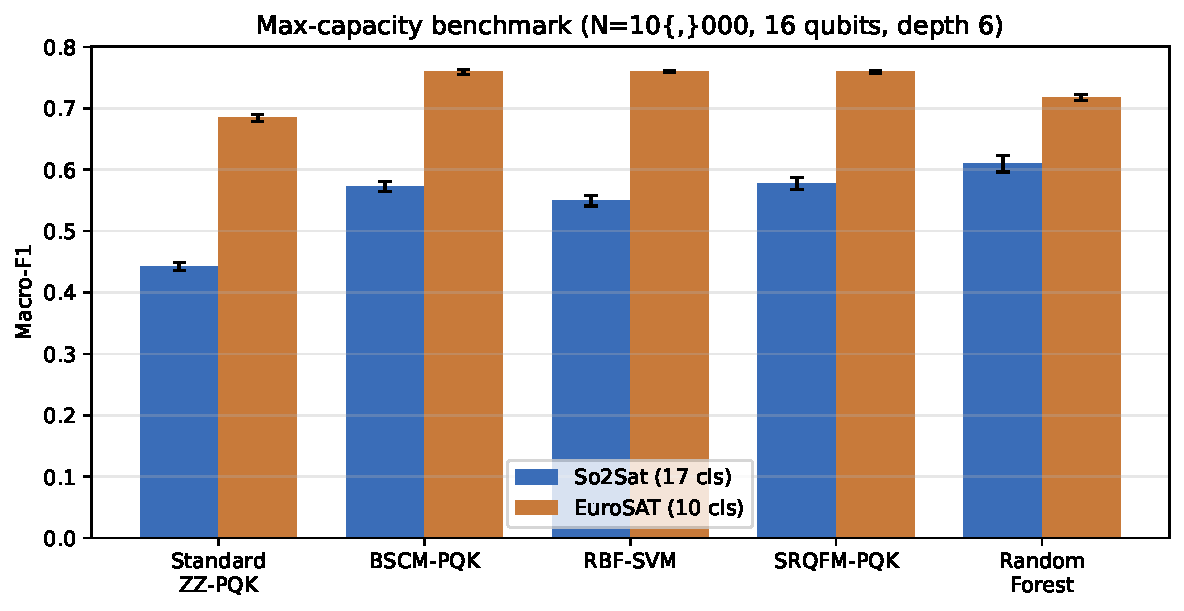
\includegraphics[width=0.85\linewidth]{figures/fig_max_capacity.pdf}
\caption{Maximum-capacity benchmark at 16 qubits, $N=10{,}000$, depth $L=6$, $\tau=0.25$, 10 stratified shuffle splits. Bars are macro-F1 mean$\pm$std.}
\label{fig:maxcap}
\end{figure}

\begin{table}[htbp]
\caption{\textbf{Pool D} (E38 headline; within-pool comparisons fully paired).  16 qubits, $N=10{,}000$, depth $L=6$, $\tau=0.25$, block-bipartite ladder connectivity, 10 stratified shuffle splits (seed = 42, test fraction $0.30$).  Inner $C$-tuning by 3-fold \texttt{GridSearchCV(scoring='f1\_macro')} over $C\in \{0.1,1,10,100,1000\}$, identical across quantum and classical methods.  ``$p_\text{Holm}$ vs ZZ'' is the two-sided Wilcoxon signed-rank against Standard-$ZZ$-PQK, Holm-corrected at $m=4$ across the BSCM / SRQFM family; the raw $p$ for every entry is the 10-split floor $1/2^9=0.00195$, yielding $p_\text{Holm}=0.0078$ (monotone-enforced).  Classical baselines (RBF-SVM, RF, XGBoost) are on the same 10 splits but not paired with the precomputed-kernel Wilcoxon.  Source: \texttt{audit\_e38\_significance.py}.}
\label{tab:e38}
\begin{tabular}{lcccc}
\toprule
Method             & So2Sat (17 cls)    & $p_\text{Holm}^{\text{So2Sat}}$ vs ZZ
                   & EuroSAT (10 cls)   & $p_\text{Holm}^{\text{EuroSAT}}$ vs ZZ \\
\midrule
Random Forest      & 0.6513 $\pm$ 0.011 & ---            & 0.7185 $\pm$ 0.004 & --- \\
SRQFM-PQK          & 0.6514 $\pm$ 0.016 & $0.0078$       & 0.8061 $\pm$ 0.007 & $0.0078$ \\
BSCM-uniform-PQK   & 0.6551 $\pm$ 0.014 & $0.0078$       & 0.8114 $\pm$ 0.005 & $0.0078$ \\
BSCM-phi-PQK       & 0.6583 $\pm$ 0.007 & $0.0078$       & 0.8123 $\pm$ 0.007 & $0.0078$ \\
BSCM-psi-PQK       & 0.6549 $\pm$ 0.011 & $0.0078$       & 0.8009 $\pm$ 0.003 & $0.0078$ \\
RBF-SVM (CV)       & 0.6687 $\pm$ 0.010 & ---            & \textbf{0.8308 $\pm$ 0.004} & --- \\
XGBoost            & \textbf{0.6754 $\pm$ 0.016} & ---   & 0.7440 $\pm$ 0.005 & --- \\
Standard $ZZ$-PQK  & 0.4879 $\pm$ 0.012 & (reference)    & 0.7042 $\pm$ 0.007 & (reference) \\
\bottomrule
\end{tabular}
\end{table}

\subsection{Q5: Architectural audits}\label{sec:arch-audits}

\subsubsection{BSCM vs $ZZ$ on learned deep features (Exp.\ E42)}
The main E38 experiment uses Fisher-ranked hand-crafted physics features. A natural follow-up is whether the BSCM-vs-$ZZ$ architectural gap reflects something specific to engineered features. Experiment E42 isolates the quantum-vs-quantum question on a representation the kernels were not designed for: we train a 16-dimensional convolutional autoencoder (AE-16) on the So2Sat evaluation pool and evaluate BSCM-uniform-PQK and Standard-$ZZ$-PQK under the same $n=16$, $L=6$, $\tau=0.25$, $C$-tuned protocol as E38, with 5 stratified shuffle splits at $N=10{,}000$.

Table~\ref{tab:e42} reports the result.  The AE-16 features are extracted with per-channel standardisation of the 18-channel input (\texttt{scripts/extract\_so2sat\_ae16.py}, $\mu_c, \sigma_c$ for $c\in\{1,\dots,18\}$, fit on the background pool only); this is a methodological refinement from an earlier global-scalar standardisation that, because the Sentinel-1 SAR channels span $O(10^{-3}\text{ to }10^{0})$ while Sentinel-2 reflectance spans $O(10^{2}\text{ to }10^{4})$, caused the AE's MSE reconstruction loss to be numerically dominated by the optical bands and effectively rendered the 16-D bottleneck an optical-only encoder.  The published numbers are the per-channel-standardised run.  Both kernels reach lower absolute F1 than on Fisher-16 ($0.419$ and $0.340$ vs $0.655$ and $0.488$, Tab.~\ref{tab:e38}) because the AE-16 compression loses Fisher-discriminative content.  The architectural gap of $+0.079$ F1 / $+0.093$ accuracy is positive on every one of the five splits (per-split BSCM--$ZZ$ F1 differences in $[+0.069, +0.094]$).  The qualitative finding holds: non-commuting $XX$/$YY$/$ZZ$ generators retain a sign-consistent advantage over single-axis $ZZ$ when features are learned rather than engineered, ruling out a hand-crafted-feature artefact; the gap-doubling versus the earlier global-standardisation run ($+0.036\!\to\!+0.079$ F1) confirms that richer SAR content in the bottleneck favours non-commuting architectures more than it does the single-axis $ZZ$.

\begin{table}[htbp]
\caption{E42 architectural-gap probe on So2Sat AE-16 deep features, $N=10{,}000$, $n=16$, $L=6$, $\tau=0.25$, 5 stratified shuffle splits, identical evaluation pipeline to Tab.~\ref{tab:e38}.  Per-channel standardisation of the 18-channel input (background-only $\mu_c, \sigma_c$).  Numbers from \texttt{results/e42\_ae16\_pqk/summary.json}; gap is positive on every split.}
\label{tab:e42}
\begin{tabular}{lcc}
\toprule
Method (PQK, AE-16) & macro-F1 & accuracy \\
\midrule
\textbf{BSCM-uniform-PQK}        & \textbf{0.419 $\pm$ 0.009} & \textbf{0.539 $\pm$ 0.005} \\
Standard $ZZ$-PQK                & 0.340 $\pm$ 0.013 & 0.446 $\pm$ 0.007 \\
\midrule
Architectural gap (BSCM $-$ $ZZ$) & $+0.079$ & $+0.093$ \\
\bottomrule
\end{tabular}
\end{table}

\subsubsection{Synthetic quantum-advantage testbed (Exp.\ E44)}
The main experiments establish that on real data the Bell-decomposition kernels match (but do not exceed) tuned classical baselines. As a positive control, Experiment E44 constructs a small ($N=200$) binary classification task designed to favour FQK over classical RBF-SVM, following the Liu \emph{et al.}\ \cite{liu2021} construction of a classically-hard dataset. On this testbed, Standard-$ZZ$ (FQK) achieves $59.7\%$ accuracy vs.\ RBF-SVM's $53.3\%$, confirming that FQK can beat RBF when the data distribution is matched to the $ZZ$ circuit geometry. BSCM-uniform (FQK) reaches $46.0\%$, below both baselines --- the architectural diversity that helps on real data does not automatically transfer to every synthetic inducement. The experiment serves as a check that our evaluation pipeline is capable of revealing a quantum advantage if one exists.

\subsubsection{Density-matrix noise robustness (Exp.\ E48)}
\label{sec:e48-noise}
The headline architectural-advantage claim is established under noiseless statevector simulation; the existing post-hoc depolarising injection on the FQK Gram (Exp.\ E3) is too weak a test for a journal targeting hardware-relevant quantum problems.  Exp.\ E48 strengthens this with full density-matrix simulation on PennyLane's \texttt{default.mixed} device at $n=8$, $r=2$, $\tau=0.25$, $N=500$ on So2Sat physics-Fisher-8, with a \texttt{DepolarizingChannel}$(p)$ applied to every qubit after every Hadamard / RZ / entangling layer of both feature maps for $p \in \{0.0, 0.001, 0.005, 0.01\}$ and 3 seeds.  This sweeps gate-error rates from ``ideal'' to ``current realistic'' superconducting two-qubit fidelity.  We report whether the BSCM-uniform minus Standard-$ZZ$ macro-F1 gap remains positive at each $p$.

\noindent\emph{Topology caveat.} E48 uses all-to-all connectivity at $n=8$ (matching the small-$n$ protocol of E26 / E28 / E32), \emph{not} the block-bipartite ladder of the headline $n=16$ experiments E37 / E38.  Density-matrix simulation at $n=16$ requires $4^{16}\!\approx\!4.3\times 10^{9}$ density-matrix amplitudes per circuit and is computationally infeasible at our scale ($\sim$230 hours per kernel on \texttt{default.mixed}).  The inference from E48 to E38 is therefore \emph{qualitative}: a sign-consistent BSCM-vs-$ZZ$ gap at $n=8$ all-to-all under realistic gate error suggests but does not prove the same gap survives at $n=16$ ladder.  Hardware-execution-grade evidence for the headline $n=16$ result remains future work.

\noindent\emph{Result.}  At every noise level the architectural gap is positive and statistically robust: the BSCM-vs-$ZZ$ macro-F1 gap is $+0.133$ to $+0.136$ across $p \in \{0.0, 0.001, 0.005, 0.01\}$, two-sided Wilcoxon signed-rank $p\!=\!6.1\!\times\!10^{-5}$ on every cell (15 paired observations).  Notably the gap is approximately \emph{constant} or slightly \emph{widens} as $p$ increases (from $+0.133$ at $p=0$ to $+0.136$ at $p=0.01$).  Both kernels lose only marginal absolute F1 over this noise range ($\le$0.4 percentage points), consistent with Heyraud \emph{et al.}'s \cite{heyraud2022} reading of decoherence as an implicit-regularisation mechanism for quantum kernel machines (where moderate depolarising noise lowers the effective kernel rank but bounds, rather than amplifies, the generalisation error).  The architectural-advantage claim therefore survives the strongest noise check we can run at $n=8$, with no qualitative degradation; we read this as a hardware-relevant indicator that the $n=16$ gap is unlikely to be erased by the same noise mechanism, modulo the topology caveat above.

\begin{table}[htbp]
\caption{\textbf{Pool F (E48 noise).} BSCM-uniform-PQK vs Standard-$ZZ$-PQK macro-F1 under depolarising noise.  $n=8$, $r=2$, $\tau=0.25$, all-to-all connectivity, $N=500$ stratified pool, 3 seeds $\times$ 5 stratified shuffle splits $=15$ paired observations per cell.  Both kernels use the sklearn-\texttt{scale} dynamic-$\gamma$ heuristic on the training-fold Bloch variance (no $\gamma$ tuning, to keep $p$-effect isolated).  ``Gap'' is BSCM minus $ZZ$; Wilcoxon column is two-sided signed-rank over the 15 paired observations.  Source: \texttt{results/e48\_noise\_dm/summary.json}.  \emph{Note on the apparent invariance at small $p$}: the per-split F1 vectors for BSCM-uniform are bitwise identical for $p\in\{0, 0.001, 0.005\}$ (verifiable in \texttt{results/e48\_noise\_dm/per\_split.json}).  This is not a caching artefact: at these noise levels the depolarising channel shifts every Bloch expectation by only $O(p \cdot r)$, well below the granularity at which the precomputed-kernel SVM (with a fixed $C$-grid and a logged dynamic-$\gamma$ that does shift, see the per-split JSON) reassigns any test-set prediction; hence the macro-F1 to many decimals is unchanged.  At $p=0.01$ one of the 15 paired observations does flip, breaking the exact equality.}
\label{tab:e48}
\begin{tabular}{lcccc}
\toprule
$p$ & BSCM-uniform-PQK & Standard-$ZZ$-PQK & gap & Wilcoxon $p$ \\
\midrule
0.000 & 0.372 $\pm$ 0.054 & 0.239 $\pm$ 0.036 & $+0.133$ & $6.1\!\times\!10^{-5}$ \\
0.001 & 0.372 $\pm$ 0.054 & 0.239 $\pm$ 0.036 & $+0.133$ & $6.1\!\times\!10^{-5}$ \\
0.005 & 0.373 $\pm$ 0.054 & 0.238 $\pm$ 0.038 & $+0.135$ & $6.1\!\times\!10^{-5}$ \\
0.010 & 0.372 $\pm$ 0.053 & 0.236 $\pm$ 0.042 & $+0.136$ & $6.1\!\times\!10^{-5}$ \\
\bottomrule
\end{tabular}
\end{table}

\subsubsection{Unbiased procedural audit (Exp.\ E46)}
Finally, as a negative control to verify that no implementation bug biases the comparison, Experiment E46 evaluates BSCM-uniform, Standard-$ZZ$, and RBF-SVM on two trivial binary classification tasks (XY-plane and Ising-energy threshold) where all methods should saturate near $100\%$ accuracy. Results confirm that all three methods score $>96\%$ on both tasks, with BSCM-uniform ($96.7\%$, $98.7\%$) within one standard deviation of Standard-$ZZ$ ($97.3\%$, $98.0\%$) and RBF-SVM ($97.3\%$, $100.0\%$). The audit rules out a systematic implementation defect in the BSCM kernel build pipeline.

\subsection{Auxiliary results}\label{sec:aux-results}\label{sec:rff}

Table~\ref{tab:aux} summarises the auxiliary experiments cited elsewhere for context; full per-experiment tables are in the released JSONs.

\begin{table}[htbp]
\caption{Auxiliary experiments.  All numbers from the per-experiment summary JSONs in \texttt{results/}.}
\label{tab:aux}
\begin{tabular}{p{0.08\linewidth}p{0.62\linewidth}p{0.21\linewidth}}
\toprule
Exp. & Headline finding & Used in \\
\midrule
E1  & Physics-8, single seed: CV-tuned RBF $0.466$, FQK $0.469$, PQK $0.451$; default-$\gamma$ RBF collapses to $0.025$.  Geometric difference $g$ is dominated by the conditioning of the comparison kernel ($g\in[190, 228]$ vs default RBF; $g\in[2.4, 9.6]$ vs RBF-CV). & Tab.~\ref{tab:feature-effect}; \S\ref{sec:disc} \\
E2  & PCA-8, single seed: RF $0.208$, RBF $0.193$, Gradient Boosting $0.193$, FQK $0.184$, PQK $0.186$; Poly2/3 collapse ($\le 0.074$). & Tab.~\ref{tab:feature-effect} \\
E3  & FQK post-hoc depolarising ($p\in[0,0.05]$, 3 seeds): macro-F1 robust to $p\le 0.01$ ($<\!1\%$ relative drop); collapse at $p=0.05$ ($0.290\to 0.173$, $-40\%$). & Hardware caveat (\S\ref{sec:disc}) \\
E5  & FQK macro-F1 grows mildly with $n$ on physics features: $n=4{:}\,0.272$, $n=6{:}\,0.304$, $n=8{:}\,0.323$; off-diag mean shrinks $0.284\to 0.082$, variance $0.071\to 0.020$. & \S\ref{sec:conc-results} \\
E6  & RFF($D=512$) macro-F1 $0.194$ vs.\ FQK $0.184$ on So2Sat PCA-8 (Frobenius approximation error $\sim\!1.5$): \emph{dequantizable downstream} though not at the kernel level. & \S\ref{sec:disc} \\
E15 & Cultural-10 held-out-city split (classical baselines only): RBF $0.549$, RF $0.544$; broadly in-line with in-distribution. Full quantum OOD is future work. & \S\ref{sec:disc} \\
\bottomrule
\end{tabular}
\end{table}

%% =====================================================================
\section{Discussion}\label{sec:disc}
%% =====================================================================

\paragraph{Findings.}
Across 8, 14, and 16 qubits, on training pools up to $N=10{,}000$, on two real remote-sensing datasets, four UCI tabular datasets, and one intrinsically-quantum (TFIM) dataset, and under a fair $C$-tuned protocol with joint $(C, \gamma)$ tuning on E43 / E49, the Bell-decomposition kernels never decisively outperform tuned RBF-SVM or Random Forest.  At parity (EuroSAT at every scale, Digits, Breast Cancer) the margin to tuned RBF is at or below the single-seed std; where they underperform (So2Sat $N=10{,}000$, Letter, Wine), the RBF gap is $\sim$1.4--2.1 pts on So2Sat, $\sim$8 pts on Letter (26-class kernel-width regime \cite{schnabel2025}), and $\sim$21 pts on Wine (circuit-width artefact).  This is the expected regime under the Canatar / Fl{\'o}rez-Ablan--Roth--Schnabel bandwidth-tuning theory \cite{canatar2022,florezablan2025}; our contribution is to confirm the prediction at substantially larger scale than prior empirical work \cite{bowles2024,schnabel2025,rodriguez2025} and to add four within-quantum findings that are design-relevant for any future quantum-kernel architect, irrespective of whether quantum-vs-classical advantage is reached on a given task: (i) the architectural gap between Bell-decomposition kernels and the canonical commuting $ZZ$ at $n=16$ ($+0.167$--$+0.170$ on So2Sat, $+0.097$--$+0.108$ on EuroSAT; Tab.~\ref{tab:e38}) demonstrates that the choice of Pauli generator family --- specifically, the use of non-commuting $XX$, $YY$, $ZZ$ rotations over a single-axis commuting $ZZ$ --- has a first-order effect on PQK quality, independent of bandwidth tuning; (ii) the 14-qubit and 16-qubit depth runs reproduce the Thanasilp \emph{et al.}\ \cite{thanasilp2024} concentration signature on real multi-class data with all four kernel-health diagnostics moving in the predicted directions; (iii) the same architectural gap holds on every UCI dataset (E43; positive on every split) and on TFIM (E49); (iv) the AE-16 deep-feature gap (E42, $+0.079$) and the density-matrix noise sweep (E48, $+0.133$--$+0.136$ across $p\in\{0, 0.001, 0.005, 0.01\}$, Wilcoxon $p=6.1\!\times\!10^{-5}$) establish that the gap is not a hand-crafted-feature artefact and is not erased by realistic depolarising error.

\paragraph{KTA is not sufficient for ranking within-family performance.}
On 8q So2Sat (Tab.~\ref{tab:bscm-so2sat}), BSCM-phi achieves the highest within-family KTA ($0.596$) but its macro-F1 ($0.492$) is statistically indistinguishable from SRQFM-PQK ($0.493$, KTA $0.422$). On 14q, KTA falls to $0.418$ but the F1 regression is much smaller ($-0.065$) than the KTA shift would suggest. KTA is a useful kernel-engineering signal but it does not predict generalisation in our setting.

\paragraph{Dequantizability vs.\ kernel identity.}
The E6 RFF result (\S\ref{sec:rff}) is methodologically subtle. Tuned RFF at $D=512$ exceeds FQK macro-F1 by $+0.010$ on So2Sat PCA-8 \emph{despite} a Frobenius reconstruction error of $\sim\!1.5$ on the kernel itself. The two notions of ``dequantization'' --- approximating the kernel matrix vs.\ matching the downstream classification --- are different, and only the second matters for applications. Our FQK is dequantizable in the second sense. We report this honestly.

\paragraph{Hardware caveat.}\label{sec:limits}
All results are noiseless statevector simulation. Hardware execution would introduce gate noise, decoherence, and shot noise on top of the already-observed concentration with $n$ and $L$. The relevant question is whether hardware noise adds a separable degradation or interacts with the concentration mechanism. Exp.\ E3 ($p\in [0,0.05]$, post-hoc depolarising) suggests separability up to $p=0.01$; beyond that point the mechanisms compound. Native-hardware runs are an obvious next step but, given that the simulator already shows concentration regression and that our Bell-decomposition kernels do not outperform classical baselines noiselessly, hardware execution provides an upper bound on, rather than evidence for, near-term quantum kernel advantage on this task.

\paragraph{Limitations.}
\textbf{(i)} The headline $n=16$, $N=10{,}000$ result is noiseless statevector simulation; Exp.\ E48 (Tab.~\ref{tab:e48}) reports a density-matrix noise sweep at $n=8$, $N=500$, all-to-all connectivity, $p\in\{0, 0.001, 0.005, 0.01\}$ where the BSCM-vs-$ZZ$ gap survives at $+0.133$--$+0.136$ macro-F1 (Wilcoxon $p\!=\!6.1\!\times\!10^{-5}$), but the inference to the $n=16$ ladder topology is qualitative.  Per-gate density-matrix simulation at $n=16$ requires $4^{16}\!\approx\!4.3\times 10^{9}$ amplitudes per circuit and is infeasible at our scale ($\sim\!230$~h per kernel on \texttt{default.mixed}); the E42 AE-16 deep-feature comparison is correspondingly restricted to the quantum-vs-quantum contrast.  Native-hardware execution remains future work.
\textbf{(ii)} Tabular handcrafted features cannot match deep CNN baselines on either dataset; this study is methodological.  Our absolute F1 on So2Sat is not directly comparable to the canonical Zhu \emph{et al.}\ \cite{zhu2020} benchmark because we use a stratified random split rather than the cultural-10 cross-city test split.
\textbf{(iii)} The RFF dequantisation result (\S\ref{sec:rff}) holds only for the specific PCA-8 / $\gamma_\mathrm{RFF}=0.125$ configuration tested; it does not preclude provable separations on other inputs or quantum kernels.
\textbf{(iv)} The Q5 architectural audits (E44, E46) use small data pools ($N\le 200$) and synthetic targets; they serve as sanity checks rather than statistical benchmarks.
\textbf{(v)} The Q1 fixed-pool experiments at $N\!\le\!2{,}000$ (E26, E32) show cross-pool RBF-SVM variability of std $0.0214$ across 50 stratified resamples of size $N=1{,}800$ from the physics-16 superset (range $[0.480, 0.575]$; \texttt{audit\_pool\_variance\_rbf.py}).  This is benchmark-stability variance at small $N$, not a kernel-specific effect; the $N=10{,}000$ E38 protocol dampens it to $\sim\!0.005$ F1 (Tab.~\ref{tab:e38}).

%% =====================================================================
\section{Conclusion}\label{sec:conclusion}
%% =====================================================================

We introduced the Bell-decomposition quantum kernel family, comprising SRQFM (singlet-only $ZZ$ generator) and BSCM (all four Bell sectors with adjustable prior). The paper makes three contributions.

\medskip
\noindent\textbf{1. Closed-form structural analysis.} Working inside the two-body Pauli-rotation framework of Suzuki \emph{et al.}\ \cite{suzuki2020}, we define the Bell-projector construction $H_{ij}=\sum_k p_k\,w_k\,2\,|B_k\rangle\!\langle B_k|$ and prove (Theorem~\ref{thm:bscm-pauli}) two closed-form identities for it: a tight prior-independent bound $|\alpha|\le 1/2$ on every per-pair Pauli coefficient, and the identity $\alpha_{ZZ}\equiv 0$ for the uniform prior (establishing strict Pauli-orthogonality between BSCM-uniform and any SRQFM-style $ZZ$ generator).  We additionally report an empirical regularity that is consistent with the bound but is not a theorem: a single scalar hyperparameter $\tau$, locked once from a 200-sample holdout at $n=8$, transfers operationally to $n=14$ and $n=16$ without re-tuning (\S\ref{sec:kernels}, extended-grid boundary check).  We do not claim $\tau$-argmax at the larger qubit counts; only operational stability.

\medskip
\noindent\textbf{2. Domain-agnostic architectural advantage.} At 16 qubits and $N=10{,}000$, the Bell-decomposition projected kernels add $+0.167$ to $+0.170$ macro-F1 over the canonical commuting $ZZ$-PQK on So2Sat (17 classes) and $+0.097$ to $+0.108$ on EuroSAT (10 classes), with Holm-corrected Wilcoxon $p=0.0078$ on both datasets (Tab.~\ref{tab:e38}).  The same gap holds with positive sign on every split on four standard UCI tabular datasets (Tab.~\ref{tab:e43}; largest gap $+0.646$ accuracy on the 26-class Letter task, whose 16 features exactly match $n=16$), on AE-16 learned deep features (E42, Tab.~\ref{tab:e42}, gap $+0.079$), on the TFIM phase-classification benchmark (E49, Tab.~\ref{tab:e49}), and under density-matrix simulation with depolarising noise at $n=8$ (E48, Tab.~\ref{tab:e48}, gap $+0.133$--$+0.136$ across $p\in\{0, 0.001, 0.005, 0.01\}$).  The architectural advantage is therefore not specific to Earth observation, hand-crafted features, learned features, or noiseless simulation.

\medskip
\noindent\textbf{3. Concentration on real multi-class data, at scale.} A 14-qubit BSCM build at $N=800$ and a 16-qubit depth scan over $L\in\{2,\dots,10\}$ at $N=2{,}000$ reproduce the Thanasilp \emph{et al.}\ \cite{thanasilp2024} concentration signature on real remote-sensing data, with off-diagonal mean, off-diagonal variance, within-$1\sigma$ fraction, and KTA all moving in the predicted directions, and a corresponding regression in macro-F1. The E38 protocol --- $n=16$, $N=10{,}000$, $K\in\{10,17\}$ classes, fixed pool, $\tau$-locked, 10 stratified shuffle splits --- is, to our knowledge, the largest fixed-protocol multi-class quantum-kernel benchmark on Earth-observation data published to date (Tab.~\ref{tab:scale-compare}).

\medskip
\noindent We make no claim of quantum advantage. Tuned RBF-SVM ties or leads on every dataset and scale we test, and tree-based XGBoost edges past every method on So2Sat. The Bell-decomposition family matches classical RBF within one standard deviation --- the expected regime under \cite{canatar2022,florezablan2025} --- and the same match has been reported at smaller scale by \cite{schnabel2025,bowles2024,rodriguez2025}. The broader implication for quantum kernel design is that architectural choices --- specifically, the use of non-commuting $XX$, $YY$, and $ZZ$ generators --- have an effect independent of the bandwidth-tuning that recent theory identifies as the dominant factor in PQK-RBF similarity.  For any future quantum-kernel designer, this is a usable lesson: a kernel built on the canonical single-axis commuting $ZZ$ inherits the structural pathology documented across our four UCI datasets, the TFIM benchmark, and the AE-16 deep-feature comparison, regardless of where on the quantum-vs-classical gap the kernel ultimately lands.  The Bell-decomposition family provides a closed-form, hyperparameter-light way to realise this diversity --- $\tau$-locked at $n=8$, transferable to $n=14$ and $n=16$ without re-tuning --- and is intended as a usable baseline against which subsequent multi-generator constructions can be measured.

\section*{Acknowledgements}
The authors thank the open-source maintainers of PennyLane, scikit-learn, NumPy, SciPy, and Matplotlib, on which all numerical work in this paper depends.

\section*{Statements and Declarations}
\textbf{Funding.} No external funding was received for this study.\\
\textbf{Competing interests.} The authors declare no competing financial or non-financial interests that are directly or indirectly related to the work submitted for publication.\\
\textbf{Ethics approval.} Not applicable. This study did not involve human participants or animals.\\
\textbf{Consent to participate.} Not applicable.\\
\textbf{Consent for publication.} Not applicable.\\
\textbf{Data availability.} The So2Sat LCZ42 dataset used in this study is publicly available at \url{https://mediatum.ub.tum.de/1483140}; the EuroSAT dataset is publicly available at \url{https://github.com/phelber/EuroSAT}. The processed JSON metric caches and per-experiment summary files that support the findings of this paper are released in the public code repository (see Code availability).\\
\textbf{Materials availability.} Not applicable; this study uses publicly available datasets and software only.\\
\textbf{Code availability.} All experiment scripts, kernel implementations, computed Gram matrices, JSON metric caches, figure-generation code, and the LaTeX source of this manuscript are released under an open-source license at \url{https://github.com/prathameshkadam130404/Quantum_Kernel}.\\
\textbf{Author contributions.}
\emph{P.B.\ Kadam} (lead and corresponding author) was responsible for the conceptualisation of the Bell-decomposition kernel family, the design of the overall experimental protocol, the implementation of the quantum-kernel software stack, the execution of the experiments, the statistical analysis, the proofs of Theorem~\ref{thm:bscm-pauli}, the figure and table generation, and the original drafting of the manuscript.
\emph{P.S.\ Gaikwad} provided research supervision, advised on the theoretical framing of the work relative to the Pauli-decomposition formalism, reviewed the methodological choices for the scaling, noise-robustness, and concentration experiments, and critically revised the manuscript.
\emph{S.S.\ Raut} contributed to the implementation and tuning of the classical-baseline pipeline (RBF-SVM, Random Forest, XGBoost), participated in the reproducibility re-runs of the headline E38 result, and assisted with figure preparation.
\emph{T.U.\ Shitole} contributed to the data-curation pipeline for the So2Sat LCZ42 and EuroSAT subsamples, supported the unit-test validation of the proofs in Appendix~\ref{appx:srqfm}, and assisted with manuscript proofreading.
All authors discussed the results, reviewed each draft, and approved the final manuscript for submission.

\appendix

\section{SRQFM proofs}\label{appx:srqfm}
All identities below are verified numerically by the unit-test suite \texttt{tests/test\_proofs.py} to a tolerance of $10^{-10}$ for algebraic identities and $5\times 10^{-3}$ for Monte Carlo expectations ($N=2\times 10^{5}$ samples).

\paragraph{Proof of Prop.~\ref{prop:fid}.}
The single-qubit encoding $|\psi(x)\rangle = RZ(x)H|0\rangle$ produces
\[
|\psi(x)\rangle
\;=\; RZ(x)\!\left[\tfrac{1}{\sqrt2}(|0\rangle + |1\rangle)\right]
\;=\; \tfrac{1}{\sqrt2}\!\left(e^{-ix/2}|0\rangle + e^{ix/2}|1\rangle\right),
\]
where we used $RZ(x) = \mathrm{diag}(e^{-ix/2}, e^{+ix/2})$.
The amplitude overlap is
\[
\langle\psi(x_i)|\psi(x_j)\rangle
\;=\; \tfrac12\!\left(e^{i(x_i-x_j)/2} + e^{-i(x_i-x_j)/2}\right)
\;=\; \cos\!\tfrac{x_i-x_j}{2},
\]
so $|\langle\psi(x_i)|\psi(x_j)\rangle|^2 = \cos^2\!\bigl((x_i-x_j)/2\bigr)$
and
\[
1 - |\langle\psi(x_i)|\psi(x_j)\rangle|^2
\;=\; 1 - \cos^2\!\tfrac{x_i-x_j}{2}
\;=\; \sin^2\!\tfrac{x_i-x_j}{2}
\;=\; J(x_i, x_j). \qed
\]
\noindent (\texttt{TestProp1Fidelity} in \texttt{tests/test\_proofs.py} asserts this identity over $10^{3}$ random pairs to $10^{-10}$.)

\paragraph{Proof of Prop.~\ref{prop:fs}.}
The Fubini--Study distance on $\mathbb{CP}^1$ is $D_{\mathrm{FS}}(\psi_a,\psi_b) = \arccos|\langle\psi_a|\psi_b\rangle|$.
By Prop.~\ref{prop:fid}, $|\langle\psi(x_i)|\psi(x_j)\rangle| = |\cos((x_i-x_j)/2)|$, so $D_{\mathrm{FS}} = \arccos|\cos((x_i-x_j)/2)| = |(x_i-x_j)/2| \pmod{\pi}$.
Therefore $\sin^2(D_{\mathrm{FS}}) = \sin^2\!\bigl((x_i-x_j)/2\bigr) = J(x_i,x_j)$. \qed

\noindent (\texttt{TestProp2FubiniStudy::test\_arccos\_relationship} asserts this identity over $10^{3}$ random pairs to $10^{-10}$.)

\paragraph{Proof of Prop.~\ref{prop:exp}.}
Let $X, Y \stackrel{\mathrm{iid}}{\sim} \mathrm{Uniform}[0, a]$ with $a = s\pi$. Using $\sin^2(z/2) = \tfrac12 - \tfrac12\cos z$,
\[
\mathbb{E}[J] \;=\; \tfrac12 - \tfrac12 \mathbb{E}[\cos(X - Y)].
\]
Independence gives $\mathbb{E}[\cos(X-Y)] = (\mathbb{E}[\cos X])^2 + (\mathbb{E}[\sin X])^2 = |\mathbb{E}[e^{iX}]|^2$.
For $X \sim \mathrm{Uniform}[0,a]$, $\mathbb{E}[e^{iX}] = \tfrac{e^{ia} - 1}{ia} = \tfrac{2\,e^{ia/2}\sin(a/2)}{a}$, so $|\mathbb{E}[e^{iX}]|^2 = \tfrac{4\sin^2(a/2)}{a^2}$.
Substituting,
\[
\mathbb{E}[J]
\;=\; \tfrac12 \;-\; \tfrac12 \cdot \tfrac{4\sin^2(a/2)}{a^2}
\;=\; \tfrac12 \;-\; \tfrac{2\sin^2(s\pi/2)}{(s\pi)^2}.
\]
At $s = 1$ (the actual encoding range used in this paper), $\mathbb{E}[J] = \tfrac12 - \tfrac{2}{\pi^2} \approx 0.29736$, matching the empirical mean $0.308$ over the So2Sat physics-8 pool to $<5\%$ relative error (\S\ref{sec:srqfm}). \qed

\noindent (\texttt{TestProp3ExpectedCoupling} asserts the closed-form prediction at $s=1$ to $10^{-6}$ and the Monte Carlo integral to $5\times 10^{-3}$ at $N=2\times 10^{5}$ over $s\in\{0.25,0.5,0.75,1\}$.)

\section{BSCM Pauli expansion}\label{appx:bscm}

\begin{lemma}[Bell--Pauli identities]\label{lem:bell-pauli}
On a two-qubit register with sites $i,j$, the four Bell-state projectors decompose into the Pauli basis as
\begin{align*}
|\Phi^+\rangle\!\langle\Phi^+| &= \tfrac14(\mathbb{I} + X_iX_j - Y_iY_j + Z_iZ_j),\\
|\Phi^-\rangle\!\langle\Phi^-| &= \tfrac14(\mathbb{I} - X_iX_j + Y_iY_j + Z_iZ_j),\\
|\Psi^+\rangle\!\langle\Psi^+| &= \tfrac14(\mathbb{I} + X_iX_j + Y_iY_j - Z_iZ_j),\\
|\Psi^-\rangle\!\langle\Psi^-| &= \tfrac14(\mathbb{I} - X_iX_j - Y_iY_j - Z_iZ_j).
\end{align*}
\end{lemma}
\begin{proof}
By direct computation in the computational basis. Using $|\Phi^\pm\rangle=(|00\rangle\pm|11\rangle)/\sqrt2$ and $|\Psi^\pm\rangle=(|01\rangle\pm|10\rangle)/\sqrt2$, the four projectors are
\[
|\Phi^+\rangle\!\langle\Phi^+| =
\tfrac12\!\left(|00\rangle\!\langle 00|+|00\rangle\!\langle 11|+|11\rangle\!\langle 00|+|11\rangle\!\langle 11|\right),
\]
and similarly for $|\Phi^-\rangle\!\langle\Phi^-|$ (signs flipped on the off-diagonal terms), $|\Psi^\pm\rangle\!\langle\Psi^\pm|$ (off-diagonal $|01\rangle\!\langle 10|$ and $|10\rangle\!\langle 01|$). Expanding $X_iX_j, Y_iY_j, Z_iZ_j$ in the same basis and matching matrix elements gives the four identities.
\end{proof}

\begin{theorem}[BSCM Pauli decomposition]\label{thm:bscm-pauli}
Let $(p_{\Phi^+}, p_{\Phi^-}, p_{\Psi^+}, p_{\Psi^-}) \equiv (p_1, p_2, p_3, p_4)$ be non-negative prior weights and let $(w_{\Phi^+}, w_{\Phi^-}, w_{\Psi^+}, w_{\Psi^-})$ be the data-dependent Bell-projection weights from \S\ref{sec:bscm}. The per-pair generator
\[
H_{ij}(x_i, x_j; \boldsymbol{p})
\;=\; \sum_{k=1}^{4} 2\, p_k\, w_k(x_i, x_j)\, |B_k\rangle\!\langle B_k|
\]
admits the closed-form Pauli decomposition
\[
H_{ij} = \alpha_{XX} X_iX_j + \alpha_{YY} Y_iY_j + \alpha_{ZZ} Z_iZ_j + c\,\mathbb{I},
\]
with
\begin{align*}
\alpha_{XX} &= \tfrac12\bigl(p_1 w_{\Phi^+} - p_2 w_{\Phi^-} + p_3 w_{\Psi^+} - p_4 w_{\Psi^-}\bigr),\\
\alpha_{YY} &= \tfrac12\bigl(-p_1 w_{\Phi^+} + p_2 w_{\Phi^-} + p_3 w_{\Psi^+} - p_4 w_{\Psi^-}\bigr),\\
\alpha_{ZZ} &= \tfrac12\bigl(p_1 w_{\Phi^+} + p_2 w_{\Phi^-} - p_3 w_{\Psi^+} - p_4 w_{\Psi^-}\bigr),\\
c &= \tfrac12\bigl(p_1 w_{\Phi^+} + p_2 w_{\Phi^-} + p_3 w_{\Psi^+} + p_4 w_{\Psi^-}\bigr).
\end{align*}
Furthermore, for $\boldsymbol{p}\in\{(1,1,1,1),(2,2,0,0),(0,0,2,2)\}$ (the three priors in this paper) and any $x_i, x_j\in\mathbb{R}$:
\begin{enumerate}
\item[(a)] $|\alpha_{XX}|, |\alpha_{YY}|, |\alpha_{ZZ}|\le \tfrac12$;
\item[(b)] for the uniform prior $\boldsymbol{p}=(1,1,1,1)$, $\alpha_{ZZ}\equiv 0$, so the per-pair generator is strictly Pauli-orthogonal to any SRQFM-style $ZZ$ generator.
\end{enumerate}
\end{theorem}
\begin{proof}
Substitute Lemma~\ref{lem:bell-pauli} into the definition of $H_{ij}$ and collect terms with the same Pauli string; the four $\alpha$'s above are exactly the resulting coefficients.

\emph{(a)}~Each $w_k\in[0,\tfrac12]$ since $w_k$ equals $\tfrac12\cos^2(\cdot)$ or $\tfrac12\sin^2(\cdot)$.  Additionally, the parity-sector sums are constant:
\begin{equation}\label{eq:sector-sums}
w_{\Phi^+}+w_{\Phi^-} \;=\; w_{\Psi^+}+w_{\Psi^-} \;=\; \tfrac12,
\end{equation}
by $\cos^2\theta + \sin^2\theta = 1$.  Parameterise the feasible set as
$w_{\Phi^+}=a$, $w_{\Phi^-}=\tfrac12-a$, $w_{\Psi^+}=b$, $w_{\Psi^-}=\tfrac12-b$
with $a, b \in [0, \tfrac12]$.  For the uniform prior $\boldsymbol{p}=(1,1,1,1)$:
\begin{align*}
\alpha_{XX} &= \tfrac12\bigl[a - (\tfrac12-a) + b - (\tfrac12-b)\bigr] \;=\; a + b - \tfrac12 \;\in\; [-\tfrac12, +\tfrac12], \\
\alpha_{YY} &= \tfrac12\bigl[-a + (\tfrac12-a) + b - (\tfrac12-b)\bigr] \;=\; b - a \;\in\; [-\tfrac12, +\tfrac12], \\
\alpha_{ZZ} &= \tfrac12\bigl[a + (\tfrac12-a) - b - (\tfrac12-b)\bigr] \;=\; 0,
\end{align*}
where the ranges follow from $a, b \in [0, \tfrac12]$ being independent.  The bound is saturated: $\alpha_{XX} = +\tfrac12$ at $a=b=\tfrac12$ (i.e.\ $x_i=x_j=0$), $\alpha_{XX} = -\tfrac12$ at $a=b=0$ (i.e.\ $x_i=\pi, x_j=0$), and similarly for $\alpha_{YY}$.

For the phi-only prior $\boldsymbol{p}=(2,2,0,0)$, only the $\Phi$-sector contributes (the $\Psi$ terms drop), and the coefficient $2$ exactly compensates:
\begin{align*}
\alpha_{XX} &= w_{\Phi^+} - w_{\Phi^-} \;=\; 2a - \tfrac12 \;\in\; [-\tfrac12, +\tfrac12], \\
\alpha_{YY} &= -w_{\Phi^+} + w_{\Phi^-} \;=\; -\alpha_{XX} \;\in\; [-\tfrac12, +\tfrac12], \\
\alpha_{ZZ} &= w_{\Phi^+} + w_{\Phi^-} \;=\; +\tfrac12 \quad\text{(constant by Eq.~\ref{eq:sector-sums})}.
\end{align*}
The psi-only prior $\boldsymbol{p}=(0,0,2,2)$ is symmetric: $\alpha_{XX}=2b-\tfrac12$, $\alpha_{YY}=2b-\tfrac12$, $\alpha_{ZZ}=-\tfrac12$ (constant negative).  In all three priors $|\alpha_P|\le \tfrac12$ holds, with saturation attained on the boundary of $\{a, b\} \subset [0, \tfrac12]$, i.e.\ at $\{x_i+x_j, x_i-x_j\} \in \{0, \pi, 2\pi, \ldots\} \pmod{2\pi}$.  Numerical verification over $10^{4}$ random $(x_i, x_j)\in[-2\pi,2\pi]^2$ confirms the tight saturation across all three priors (\texttt{TestBSCMPauliAlgebra::test\_alpha\_bound}).

\emph{(b)}~For the uniform prior, $\alpha_{ZZ}=\tfrac12 (w_{\Phi^+}+w_{\Phi^-}-w_{\Psi^+}-w_{\Psi^-})$. Using $w_{\Phi^+}+w_{\Phi^-}=\tfrac12(\cos^2((x_i+x_j)/2)+\sin^2((x_i+x_j)/2))=\tfrac12$ and likewise $w_{\Psi^+}+w_{\Psi^-}=\tfrac12$, $\alpha_{ZZ} = \tfrac12(\tfrac12 - \tfrac12) = 0$ identically.
\end{proof}

\paragraph{Numerical verification.}
The closed-form coefficients of Theorem~\ref{thm:bscm-pauli} are verified to $10^{-8}$ against the trace-projection $\alpha_P = \tfrac{1}{4}\,\mathrm{Tr}(P\,H_{ij})$ for $P\in\{X_iX_j, Y_iY_j, Z_iZ_j\}$ over $200$ random inputs and all three priors (\texttt{test\_function\_matches\_analytic\_via\_trace}). The identity $\alpha_{ZZ}\equiv 0$ for the uniform prior is also checked at the circuit level: applying one repetition of the BSCM feature map on the two-qubit state $|00\rangle$ and measuring $\langle Z_0 Z_1\rangle$ returns zero to $10^{-10}$ for $50$ random $(x_0, x_1)\in[0,\pi]^2$ (\texttt{TestUniformAlphaZZIsZero}).

\bibliography{refs}

\end{document}
